\documentclass{article}
\usepackage[fontset=fandol,UTF8]{ctex}

 \usepackage[preprint]{neurips_template}


 
    
\usepackage{hyperref}       
\usepackage{url}            
\usepackage{booktabs}       
\usepackage{amsfonts}       
\usepackage{nicefrac}       
      
\usepackage{xcolor}         


\usepackage{amsmath}
\usepackage{amssymb}
\usepackage{mathtools}
\usepackage{amsthm}
\usepackage{cases}

\usepackage{algorithm}
\usepackage{algorithmic}

\usepackage{thmtools}
\usepackage[capitalize,noabbrev]{cleveref}
\usepackage{enumitem}
\usepackage[most]{tcolorbox}
\usepackage{multirow}
\theoremstyle{plain}
\newtheorem{theorem}{Theorem}[section]
\newtheorem{proposition}[theorem]{Proposition}
\newtheorem{lemma}[theorem]{Lemma}
\newtheorem{corollary}[theorem]{Corollary}
\theoremstyle{definition}
\newtheorem{definition}[theorem]{Definition}
\newtheorem{assumption}[theorem]{Assumption}
\theoremstyle{remark}
\newtheorem{remark}[theorem]{Remark}

\crefname{definition}{Definition}{Definitions}
\crefname{assumption}{Assumption}{Assumptions}
\crefname{proposition}{Proposition}{Propositions}
\crefname{lemma}{Lemma}{Lemmas}
\crefname{corollary}{Corollary}{Corollaries}
\crefname{remark}{Remark}{Remarks}


\newcommand{\todo}[1]{\textcolor{red}{\textbf{[TODO: #1]}}}
\newcommand{\pmdmean}{\textsc{PMD-mean}}
\newcommand{\pmdpart}{\textsc{PMD-part}}
\newcommand{\KL}{\mathrm{KL}}
\newcommand{\TV}{\mathrm{TV}}
\newcommand{\E}{\mathbb{E}}
\newcommand{\Var}{\mathrm{Var}}
\newcommand{\cW}{W} 
\DeclareMathOperator*{\argmax}{argmax}
\DeclareMathOperator*{\argmin}{argmin} 
\newcommand{\abs}[1]{\left|#1\right|}
\newcommand{\norm}[1]{\left\lVert#1\right\rVert}


\title{策略镜像下降中对数配分函数的近似在大语言模型后训练中诱导了隐式正则化}




\author{%
  Zhenghao Xu\textsuperscript{1}\thanks{Work done during internship at Amazon. Emails: \texttt{\{zhenghaoxu,tourzhao\}@gatech.edu}}
  ~~~
  Qin Lu\textsuperscript{2}
  ~~~
  Changlong Yu\textsuperscript{2}
  ~~~
  Tuo Zhao\textsuperscript{1} 
  \\
\textsuperscript{1}Georgia Institute of Technology\quad 
\textsuperscript{2}Amazon
}


\begin{document}


\maketitle


\begin{abstract}
策略镜面下降（PMD）通过迭代求解带有KL正则化的策略改进子问题，为强化学习（RL）提供了一个合理的框架。尽管该方法已被用于训练先进的大模型（如Kimi K1.5/K2），但理想的闭式PMD更新需要可靠的配分函数估计，在大模型庞大的动作空间中，由于可用的滚动数据有限，这一目标面临巨大挑战。

我们研究了一种实用的算法，称为 \textsc{PMD-mean}，该算法使用采样策略下的平均奖励来近似对数划分项，并在对数策略空间中进行回归。具体而言，我们刻画了 \textsc{PMD-mean}\ 的总体解，并证明其隐式地优化了带有自适应混合 KL--$\chi^2$  正则化项的镜面下降子问题。这一额外的 $\chi^2$  正则化项限制了概率的大幅变化，在期望奖励较低时产生更保守的更新，从而增强了对有限样本估计误差的鲁棒性。

数学推理任务的实验表明，\textsc{PMD-mean}\ 在性能、稳定性和时间效率方面均表现出色。这些发现深化了我们对 \textsc{PMD-mean}\ 的理解，并为大模型强化学习算法的系统性改进指明了方向。代码可在 \url{https://github.com/horizon-rl/OpenKimi}. 处获取。
\end{abstract}

\section{引言}
\label{sec:intro}

强化学习（Reinforcement Learning, RL）已成为提升大模型（Language Model, LLMs）在推理任务和Agentic目标上后训练的标准范式 \citep{jaech2024openai,guo2025deepseek}。尽管实现方式多样，大多数RL算法都可以形式化为 \emph{正则化策略改进}（regularized policy improvement），这是一种迭代方法，通过最大化奖励同时保持与参考策略的接近性来更新策略。

策略镜面下降（Policy Mirror Descent, PMD, \citealt{geist2019theory,tomarmirror}）通过迭代求解KL正则化改进子问题，为该方法提供了正则的公式化表达。理论上，这些子问题具有优美的闭式解，通过重新加权当前策略并使用配分函数进行归一化来实现。然而，在实践中，可靠估计该配分函数，并从有限的轨迹中拟合理想目标，带来了显著挑战，尤其是在大型动作空间的LLM后训练场景中。

求解KL正则化子问题的一种常见方法是直接对正则化目标应用策略梯度方法 \citep{williams1992simple}，通过将正则化项融入奖励函数或显式添加KL惩罚项来实现。TRPO \citep{schulman2015trust}、PPO \citep{schulman2017proximal}、RLOO \citep{ahmadian2024back} 和 GRPO \citep{shao2024deepseekmath} 等方法利用滚动样本构建替代损失，在滚动样本来自当前策略时（即同策略情况下）表现最优。

然而，现代高效的强化学习实现越来越多地利用大规模生成批次或异步回放，以防止长尾生成带来的计算瓶颈 \citep{noukhovitch2024asynchronous,fu2025areal}。  
这些方法通常会带来一个\emph{过时代价}：采样策略滞后于正在更新的策略，从而造成根本性的训练/推理不匹配。这种不匹配引入了稳定性问题，从业者通常通过重要性加权并结合裁剪或其他启发式方法来缓解 \citep{yao2025offpolicy,liu-li-2025-rl-collapse}。尽管部分有效，但这些补救技术极大地增加了实现和理论分析的复杂性。

本文研究了一种由Kimi K1.5/K2 \citep{team2025kimik15,team2025kimik20}推广的替代极简方法，该方法从根本上重新构建了问题。与其尝试通过复杂的校正机制和启发式方法减轻异策略性，该算法采用了针对PMD的异策略回归视角。具体而言，该方法不拟合确切的划分规范化目标，而是使用采样策略下的均值奖励近似对数划分项，并直接在对数策略空间中拟合回归目标。我们将这种实用算法称为\textsc{PMD-mean}（或“Kimi风格PMD”）。

尽管在强正则化条件下，这种均值奖励近似仍保持准确，但在使用较小正则化（实践中常见）时，其结果可能与划分规范化更新产生显著偏差。这一偏差引发了一个根本性问题：

\begin{center}
\emph{\textsc{PMD-mean} 优化的确切目标是什么，该目标带来了哪些算法上的后果？}
\end{center}

\textbf{我们的结果。} 我们通过推导 \textsc{PMD-mean}\ 人群解的闭式表达，解决了这一基本问题。尽管理想的KL正则化PMD更新产生标准的玻尔兹曼权重重分配，但我们的分析表明，\textsc{PMD-mean}\ 生成的更新涉及朗伯-$W$  函数。

此外，我们证明该更新在数学上等价于使用一个\emph{混合}KL--$\chi^2$ 正则化项进行镜像下降，其中$\chi^2$ 权重根据当前策略下的平均奖励动态\emph{自适应}调整。这一额外的$\chi^2$ 项相较于仅使用KL时对概率变化施加了更强的惩罚，尤其在平均奖励较低时效果更为显著。这种自适应正则化在训练初期有效调节了收敛速率，为该算法的实验稳定性提供了合理的解释。

我们的进一步分析表明，与拟合划分规范化目标（\textsc{PMD-part}）相比，\textsc{PMD-mean} 在轨迹数量有限的情况下对有限样本误差表现出显著降低的敏感性。这一特性大幅降低了对误估计目标过拟合的风险。  
该发现为 \textsc{PMD-mean} 在实际应用中表现出的增强稳定性提供了理论解释：隐式引入的 $\chi^2$ 正则化带来了额外的鲁棒性，这在大型语言模型后训练中典型的数据受限场景下具有重要价值。

\textbf{贡献。}
我们做出了以下贡献：

$\bullet$  \textbf{关于 \textsc{PMD-mean} 的确切刻画。} 我们在策略空间中推导出 \textsc{PMD-mean} 的闭式解，并建立其与带有自适应混合 KL--$\chi^2$  正则化项的镜面下降子问题的等价性。

$\bullet$  \textbf{正则化与稳定性机制。} 我们证明，所诱导的 $\chi^2$  项提供了对概率比的额外控制，即使名义上的KL系数极小，也能提供显著的正则化作用。

$\bullet$  \textbf{收敛性分析。} 在标准假设下，我们开发了一种非精确-PMD风格的收敛性分析，该分析区分了 \textsc{PMD-mean}\ 和 \textsc{PMD-part}\ 并刻画了它们的分离。

$\bullet$  \textbf{实验验证。} 通过在数学推理任务上的实验，我们通过实证确认了 \textsc{PMD-mean} 在效率和稳定性方面的提升，同时展示了其相对于标准 GRPO 的性能优势。


\section{初步研究}
\label{sec:prelim}

为简化问题，我们将大语言模型的后训练强化学习表述为一个上下文老虎机问题。令 $x\in\mathcal{X}$ 为输入提示（状态），$y\in\mathcal{Y}$ 表示生成的响应（动作），$r(x,y)\in[0,1]$ 表示一个有界奖励函数。  
一个语言模型策略 $\pi\colon\mathcal{X}\to\Delta(\mathcal{Y})$ ，将状态映射到动作上的分布，诱导出期望奖励：
\begin{align*}
    J(\pi) \coloneqq \mathbb{E}_{x\sim\mathcal{D}} \mathbb{E}_{y\sim \pi(\cdot\mid x)} \big[r(x,y)\big],
\end{align*}
其中 $\mathcal{D}$ 是提示词的分布（例如，一个数据集）。  
在实际应用中，大语言模型策略被实现为 token-wise Softmax 分布的组合，这些分布为词表中的每个 token 分配非零概率。因此，我们可以合理地假设 $\pi$ 在所有可能响应的动作空间上具有完整的支撑，即 $\pi(y\mid x)>0$ 对所有 $x\in\mathcal{X}$ 和 $y\in\mathcal{Y}$ 成立。


\textbf{策略镜面下降。} 
在全局步 $t$ ，KL正则化策略镜面下降（PMD；\citealt{geist2019theory,tomarmirror}）通过求解以下优化问题来更新策略 $\pi_t$ ，该问题针对每个状态 $x$ ：
\begin{align}
    \pi_{t+1}(\cdot\mid x) = 
    &\argmax_{\pi(\cdot\mid x)\in \Delta(\mathcal{Y})}
    \mathbb{E}_{y\sim \pi(\cdot\mid x)}[r(x,y)]-
    \tau\cdot\text{KL}\left(\pi(\cdot\mid x)~\|~\pi_t(\cdot\mid x)\right),
    \label{eq:pmd_kl_subproblem}
\end{align}
其中 $\tau>0$ 是控制正则化强度的正则化参数。在 $\mathcal{Y}$ 上，分布 $p$ 与 $q$ 之间的 KL 散度为 $\text{KL}(p~\|~q)\coloneqq\mathbb{E}_{y\sim p}\left[\log\frac{p(y)}{q(y)}\right]$ 。

该KL正则化优化问题 \eqref{eq:pmd_kl_subproblem} 拥有如下唯一的闭式解：
\begin{align}
    \pi_{t+1}(y\mid x)
    =\frac{\pi_t(y\mid x)\exp(r(x,y)/\tau)}{Z_t(x)},
    \label{eq:boltzmann_update}
\end{align}
其中 $Z_t(x)\coloneqq \mathbb{E}_{y\sim \pi_t(\cdot\mid x)}\left[e^{r(x,y)/\tau}\right]$ 是配分函数，确保规范化。此更新类似于玻尔兹曼分布，根据奖励信号对先前策略进行指数加权。


\textbf{通过回归拟合目标。}
在动作空间较大的情况下，公式\eqref{eq:boltzmann_update}中的理想更新在计算上是不可行的，因为它需要评估配分函数并为每个动作分配概率。
一种直接的异策略方法是使用平方回归在对数策略空间中拟合目标。在收集轨迹$y\sim \pi_t(\cdot\mid x)$并评估奖励$r(x,y)$后，我们定义状态相关的目标对数比率：
\begin{align*}
    s^\star_{\mathrm{part}}(x,y)
    \coloneqq\log \frac{\pi_{t+1}(y\mid x)}{\pi_t(y\mid x)}
    = \frac{r(x,y)}{\tau} - \log Z_t(x),
\end{align*}
其中 $\pi_{t+1}$ 根据公式 \eqref{eq:boltzmann_update} 定义。  
这导致以下平方回归损失： 
\begin{align}
    &\mathcal{L}_{\mathrm{part}}(\pi)
    \coloneqq\E_{x\sim \mathcal{D}}\E_{y\sim \pi_t(\cdot\mid x)}\left[\frac{1}{2}\Big(\log \frac{\pi(y\mid x)}{\pi_t(y\mid x)} - s^\star_{\mathrm{part}}(x, y)\Big)^2\right].
    \label{eq:L_partition}
\end{align}
如果策略类能够确切表示目标分布（即满足可实现性）且 $Z_t(x)$  精确已知，则最小化 \eqref{eq:L_partition}  可恢复最优策略更新。  
然而，在实际应用中，$Z_t(x)$  必须从相同的有限集回溯轨迹中估计得到，这会引入显著的估计误差。  
对于较大的动作空间和较小的正则化参数 $\tau$ ，这种估计可能极不稳定，导致病态的更新行为（见 \Cref{sec:experiments}）。  
我们将这种直接拟合方法称为 \textsc{PMD-part}。

\textbf{\textsc{PMD-mean}: 对数配分函数的近似。}
不直接拟合 $s^\star_{\mathrm{part}}$ ，\citet{team2025kimik15} 提出一种替代方法，用平均奖励来近似对数配分函数，从而得到一个修改后的损失函数。
具体而言，我们在使用均值奖励基准的情况下，定义优势函数 $\Delta(x,y)$ 于 $\pi_t$ ：
\begin{align*}
\Delta(x,y) \coloneqq r(x,y) - \mathbb{E}_{y^\prime\sim \pi_t(\cdot\mid x)}[r(x,y^\prime)].
\end{align*}
根据此定义，回归的目标变为：
\begin{align}
    &\mathcal{L}_{\mathrm{mean}}(\pi)
    \coloneqq\E_{x\sim \mathcal{D}}\E_{y\sim \pi_t(\cdot\mid x)}\left[\frac{1}{2}\left(\log \frac{\pi(y\mid x)}{\pi_t(y\mid x)}-\frac{\Delta(x,y)}{\tau}\right)^2\right].
    \label{eq:L_mean}
\end{align}
我们将这种实用的变体称为 \textsc{PMD-mean}，该方法已被用于训练先进的模型，如 Kimi K1.5 和 K2 \citep{team2025kimik15,team2025kimik20}。  
在实际应用中，期望奖励 $\mathbb{E}_{y^\prime\sim \pi_t(\cdot\mid x)}[r(x,y^\prime)]$ 可以通过在采样响应上对每个提示进行蒙特卡罗平均来高效估计。


\section{\textsc{PMD-mean} 的隐式正则化}
\label{sec:pmdmean}

\textsc{PMD-mean}\ 所采用的近似在 $\tau\to\infty$ 时是准确的。  
然而，较大的 $\tau$ 会显著减慢收敛速度，当 $\tau$ 变小时，平均奖励与对数配分函数之间的偏差会显著增大（\Cref{fig:partition_vs_mean}，左）。  
因此，\eqref{eq:L_mean} 的解可能与 \eqref{eq:boltzmann_update} 中的理想目标 $\pi_{t+1}$ 显著不同，即使提供了无限样本（\Cref{fig:partition_vs_mean}，右），也不再对应于 KL 子问题 \eqref{eq:pmd_kl_subproblem} 的解。 


\subsection{\textsc{PMD-mean} 的确切解}
\label{sec:closed_form}
为了理解 \textsc{PMD-mean} 的实际目标，我们刻画了 \eqref{eq:L_mean} 的总体最小化器。  
为简便起见，我们省略 $x$ 并考虑单一状态，记为 $\pi_t(y)$ 和 $\Delta_y$。
\begin{theorem}[\pmdmean\ solution]
    \label{thm:pmdmean_solution}
    假设对所有 $y\in\mathcal{Y}$ 均有 $\pi_t(y)>0$。  
令 $\Delta_y \coloneqq r(y) - \E_{y^\prime\sim \pi_t}[r(y^\prime)]$ 表示均值-基准优势。  
则 \eqref{eq:L_mean} 在概率单纯形上的唯一最小化点满足
    \begin{align}
        \pi_{t+1}(y)
        =\pi_t(y)\exp\Big(\frac{\Delta_y}{\tau}-\cW\Big(\frac{\lambda}{\tau^2}\exp\Big(\frac{\Delta_y}{\tau}\Big)\Big)\Big),
        \label{eq:pmdmean_lambertW_form}
    \end{align}
    其中$\cW(\cdot)$是Lambert-$W$函数的主分支（$f(w)=w\cdot e^w$的逆函数），$\lambda\ge 0$是一个规范化常数，其选取满足$\sum_y \pi_{t+1}(y)=1$。此外，定义$A\coloneqq \E_{\pi_t}[\exp(\Delta_y/\tau)]$和$B\coloneqq \E_{\pi_t}[\exp(2\Delta_y/\tau)]$，该规范化常数满足
    \begin{align}
        \tau^2\frac{A(A-1)}{B}\leq\lambda\leq\tau^2\log A.
        \label{eq:lambda_bounds}
    \end{align}
    对于二元奖励 $r\in\{0,1\}$ 且 $p=\E_{\pi_t}[r(y)]$ ，
    \begin{align}
        \lambda\approx\begin{cases}
            \frac{1}{2}p(1-p), & \tau\to\infty\\
            \tau p(1-p), &\tau\to 0.
        \end{cases}
        \label{eq:lambda_asymptotics}
    \end{align}
\end{theorem}
通过 \Cref{thm:pmdmean_solution}，\textsc{PMD-mean}\ 的解使用朗伯-$W$ 函数对动作概率进行异质性规范化，与独立于动作 $y$ 的对数-配分函数作为规范化项的 KL 解 \eqref{eq:boltzmann_update} 相反。  
由于 $W$ 的单调性，相较于 KL 解，具有较大 $\Delta_y$  的动作其概率将被抑制，而具有较小 $\Delta_y$  的动作则不会受到如此严厉的惩罚。  
因此，\textsc{PMD-mean}\ 更新比 \textsc{PMD-part} 更为温和。 


更精确地说，假设奖励是二值的，且在 $\pi_t$  下的平均奖励为 $p$。  
我们考虑当 $\tau$  较小时，正动作与负动作上的比率 $\pi_{t+1}/\pi_t$。  
对于正动作，$r(y)=1$，\textsc{PMD-mean}\ 产生 
\begin{align}
    \frac{\pi^{\mathrm{mean}}_{t+1}(y)}{\pi_t(y)}
    =\frac{1}{p}-\frac{1-p}{p}e^{-p/\tau}(1+o(1)),
    \label{eq:ratio_pos_mean}
\end{align}
而 \textsc{PMD-part}\ 产生 
\begin{align}
    \frac{\pi^{\mathrm{part}}_{t+1}(y)}{\pi_t(y)} 
    &= \frac{1}{p} - \frac{1-p}{p^2}e^{-1/\tau} + O(e^{-2/\tau}).
    \label{eq:ratio_pos_part}
\end{align}
当两个比率在 $\tau\to 0$ 时均从下方趋近于 $1/p$，但在 $p$ 较小时（例如训练的早期阶段），\textsc{PMD-mean}\ 的差距要大得多，因此更新更加保守。  
对于负动作，分离更为明显：当 $r(y)=0$ 时，\textsc{PMD-mean}\ 产生 
\begin{align}
    \frac{\pi^{\mathrm{mean}}_{t+1}(y)}{\pi_t(y)}
    =e^{-p/\tau}(1+o(1)),
    \label{eq:ratio_neg_mean}
\end{align}
而 \textsc{PMD-part}\ 产生 
\begin{align}
    \frac{\pi^{\mathrm{part}}_{t+1}(y)}{\pi_t(y)} 
    =\frac{1}{p}e^{-1/\tau}+O(e^{-2/\tau}).
    \label{eq:ratio_neg_part}
\end{align}
当 $p$ 很小时，差异显著，如 \Cref{fig:ratio} 所示。  
完整的推导过程见 \Cref{sec:appendix-ratio}。 


\begin{figure}[t]
    \begin{center}
        \begin{minipage}[c]{0.4\columnwidth}
            \centering
            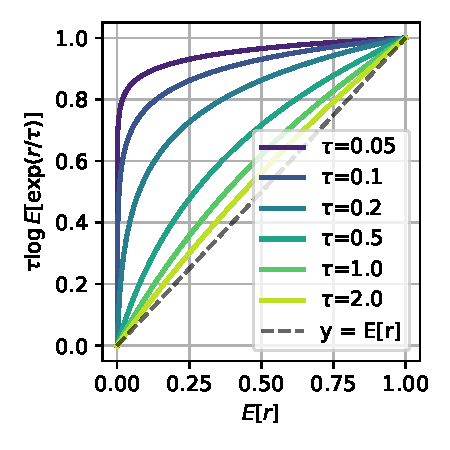
\includegraphics[width=\linewidth]{figs/fig1_thin.pdf}
        \end{minipage}
        \begin{minipage}[c]{0.35\columnwidth}
            \centering
            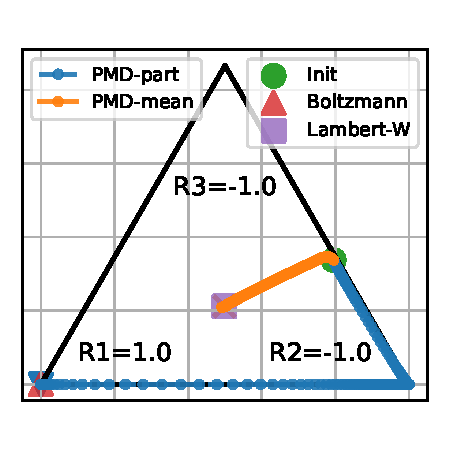
\includegraphics[width=\linewidth]{figs/fig0.pdf}
        \end{minipage}
        \vspace{-0.1in}
        \caption{
        左图：在假设二元奖励的情况下，缩放后的对数划分函数与平均奖励的关系。对于中等大小的 $\tau$ ，两者之间的差距显著。
右图：\textsc{PMD-mean}\ 和 \textsc{PMD-part}\ 在概率单纯形中收敛到不同子问题解的示意图。
        }
        \label{fig:partition_vs_mean}
    \end{center}
    \vspace{-0.1in}
\end{figure}


\subsection{\textsc{PMD-mean}\ as Mirror Descent with Mixed KL--$\chi^2$  正则化}
\label{sec:mixed_div}

Lambert-$W$ 的闭式解对分析很有用，而更直观的理解是，\textsc{PMD-mean}\ 正在\emph{确切地}解决一个不同的正则化策略改进问题。  
令 $\chi^2(p~\|~q)\coloneqq\E_{y\sim q}\big[(\frac{p(y)}{q(y)}-1)^2\big]$ 表示两个定义在 $\mathcal{Y}$ 上的分布 $p$ 和 $q$ 之间的 $\chi^2$ 散度。  
以下命题表明，\textsc{PMD-mean}\ 更新等价于带有额外 $\chi^2$ 项惩罚的镜面下降法。

\begin{proposition}[Equivalent mixed KL--$\chi^2$ subproblem]
\label{prop:mixed_subproblem}
    固定一个状态 $x$（为简洁起见省略）。
令 $\pi_{t+1}$ 为 \Cref{thm:pmdmean_solution} 中的 \textsc{PMD-mean}\ 群体解，$\lambda$ 为相同的规范化常数。
则 $\pi_{t+1}$ 为解
    \begin{align}
        \pi_{t+1}
        =&\argmax_{\pi\in\Delta(\mathcal{Y})}
        \E_{y\sim \pi}\big[r(y)\big]
        -\tau\KL(\pi~\|~\pi_t)-\frac{\lambda}{2\tau}\chi^2(\pi~\|~\pi_t).
        \label{eq:mixed_subproblem}
    \end{align}
\end{proposition}
\Cref{prop:mixed_subproblem} 直接来自于两个问题的KKT条件（参见 \Cref{sec:proof_mixed}）。  
$\chi^2$ 惩罚项直接抑制了策略比率的大幅波动，并相较于KL正则化提供了更强的正则化效果，如 $\KL(p~\|~q)\leq \chi^2(p~\|~q)$ 对 $p,q$ 具有完整支撑时所示。  
此外，\Cref{thm:pmdmean_solution} 表明有效强度 $\lambda/\tau$ 是 \emph{自适应} 的。  
对于二元奖励，即使 $\tau\to 0$ 增大，$\lambda/\tau$ 仍保持 $O(1)$，这意味着当名义上的KL正则化较小时，\textsc{PMD-mean} 依然能对更新进行正则化。

\begin{remark}[Connection to $\chi^2$ preference optimization]    
混合KL--$\chi^2$ 正则化项出现在 $\chi^2$ 正则化的偏好最优化（$\chi$ PO, \citealt{huang2024correcting}）中，为避免在KL正则化偏好最优化中的过度优化提供了可证明的保证。  
我们的结果表明，\textsc{PMD-mean}\ 可以被解释为这一思想的在线版本，其自适应系数 $\lambda$ 与采样奖励分布相关联。 
\end{remark}
\begin{remark}[Policy ratios compared to \citealt{huang2024correcting}]    
\citet{huang2024correcting} 在他们的命题4.2中表明，混合KL--$\chi^2$ 正则化问题在我们的记号下产生
\begin{align}\label{eq:huang_mixed_ratio}
    \exp\left(-\frac{R_{\max}}{\tau}\right)\lesssim\frac{\pi^\mathrm{mix}_{t+1}}{\pi_t}\lesssim 1+\frac{R_{\max}}{\tau},
\end{align}
而KL正则化问题则产生 
\begin{align}\label{eq:huang_kl_ratio}
    \exp\left(-\frac{R_{\max}}{\tau}\right)\lesssim\frac{\pi^\mathrm{KL}_{t+1}}{\pi_t}\lesssim \exp\left(\frac{R_{\max}}{\tau}\right),
\end{align}
where $r\in[0, R_{\max}]$ 是奖励的边界。  
这突出了上策略比率控制中 $1/\tau$ 的最坏情况 {多项式 vs. 指数} 对比。  
然而，这些边界在 $R_{\max}$ 上是一致的，并且在与我们的二元奖励分析相关的情形中可能是空洞的。  
特别地，\eqref{eq:huang_kl_ratio} 忽略了也随 $1/\tau$ 增长的划分归一化因子。  
相比之下，我们的情景对小 $\tau$ 呈现出显著更尖锐且分布相关的行为。  
正如 \eqref{eq:ratio_pos_mean} 和 \eqref{eq:ratio_pos_part} 所示，两个比率共享相同的常数上界 $1/p$，但趋近该上界的指数速率不同。  
因此，在我们的情景中，混合和 KL 散度之间的差距更多是分布相关的指数速率的区别，即 $O(e^{p/\tau})$ vs. $O(e^{1/\tau})$，而非多项式 vs. 指数。 
\end{remark}

\begin{figure}[t]
  \begin{center}
    \centerline{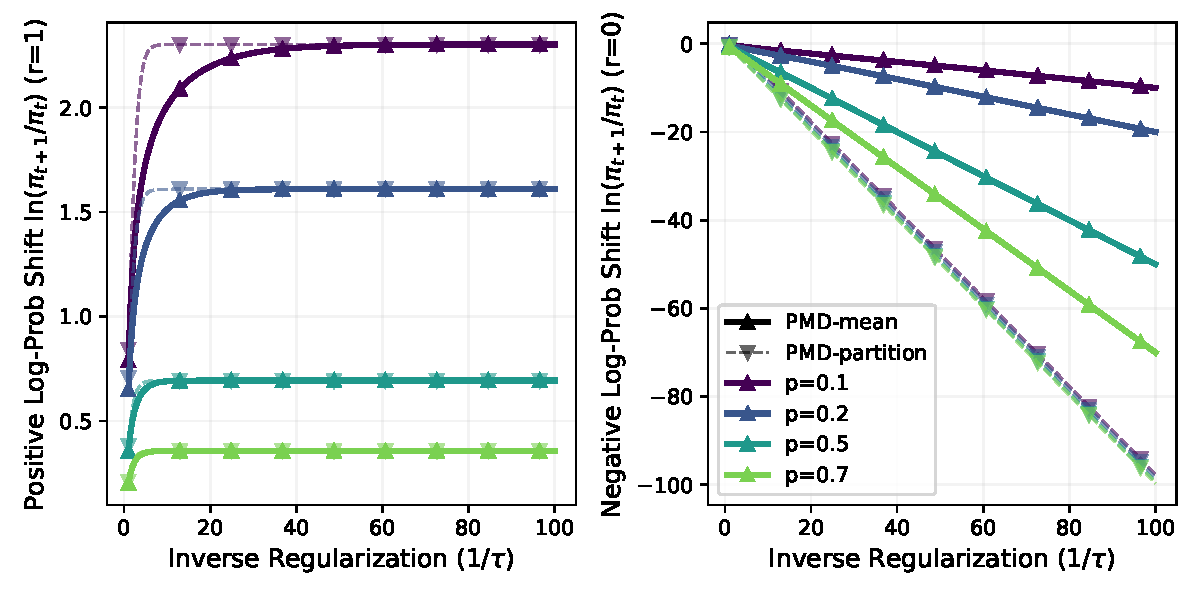
\includegraphics[width=0.75\columnwidth]{figs/change_ratio.pdf}}
    \vspace{-0.1in}
    \caption{
      \textsc{PMD-mean}\ 的更新的（对数）概率比在二元奖励情况下比 \textsc{PMD-part}\ 更为保守。 
    }
    \label{fig:ratio}
  \end{center}
  \vspace{-0.2in}
\end{figure}


\section{收敛的含义}
\label{sec:theory}
我们从回归视角提供一种不精确的PMD收敛性分析，以说明隐式正则化对收敛性的影响。  
为清晰起见，我们仍然忽略 $x$ 并仅分析一个状态。对提示分布 $x\sim\mathcal{D}$ 的平均扩展是标准的。

\subsection{一步策略改进}
\label{sec:convergence}
召回率 $J(\pi)\coloneqq \E_{y\sim \pi}[r(y)]$，其中 $r(y)\in[0,1]$。  
在迭代 $t$ 时，令 $\pi^\star_{t+1}$ 表示 \textsc{PMD-part}\ 或 \textsc{PMD-mean}\ 中的理想目标更新，  
并定义其目标对数比 $s^\star(y)\coloneqq \log\frac{\pi^\star_{t+1}(y)}{\pi_t(y)}$。  
令 $\Pi$ 为策略类，并对每个 $\pi\in\Pi$，定义 $s_\pi(y)\coloneqq \log\frac{\pi(y)}{\pi_t(y)}$。  
\textsc{PMD-part}\ 和 \textsc{PMD-mean}\ 的目标是通过最小化总体损失，用 $s_\pi$ 拟合理想目标 $s^\star$。
\begin{align}\label{eq:population-loss}
    \mathcal{L}_t(\pi)
    &\coloneqq
    \frac{1}{2}\E_{y\sim\pi_t}\big[(s_\pi(y)-s^\star(y))^2\big].
\end{align}

在实际应用中，$\pi^\star_{t+1}$ 依赖于无法确切获得的总体数量（例如 $\E_{\pi_t}[r]$ 或 $\log Z_t$），因此我们改用有限的蒙特卡洛样本构造一个估计的目标更新 $\widetilde{\pi}^\star_{t+1}$。  
给定独立同分布的样本 $y_1,\dots,y_n\sim \pi_t$，我们最小化经验损失
\begin{align}\label{eq:empirical-loss}
    \widehat{\mathcal{L}}_t(\pi)
    &\coloneqq
    \frac{1}{2n}\sum_{i=1}^n (s_\pi(y_i)-\widetilde{s}_{-i}^\star(y_i))^2,
\end{align}
其中，目标在 $y_i$  处变为留一法（LOO）估计版本 $\widetilde{s}_{-i}^\star(y_i)$ ： 
\begin{numcases}{\widetilde{s}_{-i}^\star(y_i)=}
    \frac{1}{\tau}\Bigl(r(y_i)-\frac{1}{n-1}\sum_{j\neq i}r(y_j)\Bigr) & \text{(\pmdmean)}\label{eq:loo-s-mean}\\
    \frac{r(y_i)}{\tau}-\log\Bigl(\frac{1}{n-1}\sum_{j\neq i}e^{r(y_j)/\tau}\Bigr) & \text{(\pmdpart)}\label{eq:loo-s-part}
\end{numcases}


设 $\widehat{\pi}_{t+1}$ 为近似的 ERM 解，并设 $\pi_{t+1}\coloneqq \widehat{\pi}_{t+1}$ 。  
我们作出以下假设以进行分析。 

\begin{assumption}[Realizability]
\label{asm:realizable_plugin}
    $\pi^\star_{t+1}\in\Pi$.
\end{assumption}

\begin{assumption}[Bounded optimization error]
\label{asm:opt_err}
    $\widehat{\mathcal{L}}_{t}(\widehat{\pi}_{t+1})\leq \inf_{\pi\in\Pi}\widehat{\mathcal{L}}_t(\pi)+\epsilon_{\mathrm{opt}}$.
\end{assumption}

\begin{assumption}[Bounded log-ratio]
\label{asm:bounded_logratio}
    存在 $B,B_+>0$，使得对所有 $\pi\in\Pi$ 和 $y\in\mathcal{Y}$，
    \begin{align}
        s_\pi(y)\leq B_+,
        \quad
        \abs{s_\pi(y)}\leq B.
        \label{eq:bounded_logratio_conv}
    \end{align}
\end{assumption}

\begin{assumption}[Finite policy class]
\label{asm:finite_class}
    $\abs{\Pi}<\infty$.
\end{assumption}

\Cref{asm:realizable_plugin} is standard in the 样本高效的强化学习文献 \citep{foster2023foundations}. 
\Cref{asm:opt_err} is a generic assumption that allows focusing on 统计速率 without involving overcomplicated subproblem optimization dynamics.
\Cref{asm:bounded_logratio} can be achieved by restricting the 策略类 via clipping. 
\Cref{asm:finite_class} is for simplicity, and one can extend it to general 策略类 with $\abs{\Pi}$ replaced by other complexity metrics, e.g., covering number.  
Under these assumptions, we have the following lemma that characterizes the error of the approximate 经验风险最小化(ERM)解的误差 $\widehat{\pi}_{t+1}$ . 
\begin{lemma}[Empirical minimization]\label{thm:erm_loo}
    对于全局步骤 $t$，假设 $y_1,\dots,y_n\sim\pi_t$ 为独立同分布的样本。  
令 $\mathcal{L}_t(\pi)$ 和 $\widehat{\mathcal{L}}_t(\pi)$ 分别表示在 \eqref{eq:population-loss} 和 \eqref{eq:empirical-loss} 中定义的总体损失和经验损失。  
定义目标不匹配
    \begin{align*}
        \Delta_i \coloneqq \widetilde{s}^\star_{-i}(y_i)-s^\star(y_i),
        \quad
        \overline{\Delta^2}\coloneqq \frac{1}{n}\sum_{i=1}^n \Delta_i^2.
    \end{align*}
    在 \Cref{asm:realizable_plugin,asm:opt_err,asm:bounded_logratio,asm:finite_class} 下，对于任意 $\delta\in(0,1)$ ，以至少 $1-\delta$ 的概率，
    \begin{align}
    \label{eq:erm_master_bound}
        \mathcal{L}_t(\widehat{\pi}_{t+1})
        \lesssim
        \frac{B^2\log(\abs{\Pi}/\delta)}{n} + \epsilon_{\mathrm{opt}} + \overline{\Delta^2}.
    \end{align}
\end{lemma}
证明在 \Cref{sec:proof_erm_loo} 中给出。  
随后，ERM 解的误差被转化为影响单步策略改进的 $J(\pi^\star_{t+1})$ 与 $J(\widehat{\pi}_{t+1})$ 之间的差距。 
\begin{theorem}[One-step policy improvement]
    \label{cor:convergence_one_step}
    在 \Cref{asm:realizable_plugin,asm:opt_err,asm:bounded_logratio,asm:finite_class} 下，假设理想的种群更新 $\pi^\star_{t+1}$ 满足，对于某个 $\eta_t\in(0,1]$ ，
    \begin{align}
        1 - J(\pi^\star_{t+1})
        \leq
        (1-\eta_t)\big(1-J(\pi_t)\big).
        \label{eq:ideal_improvement}
    \end{align}
    令 $\pi_{t+1}\coloneqq\widehat{\pi}_{t+1}$ 和 $\overline{\Delta^2}$ 如 \Cref{thm:erm_loo} 所定义。  
则对于 $\delta\in(0,1)$ ，以至少 $1-\delta$ 的概率，
    \begin{align}
        &1 - J(\pi_{t+1})
        \leq (1-\eta_t)\big(1-J(\pi_t)\big)+O\Big(e^{B_+/2}\Big(B\sqrt{\frac{\log(\abs{\Pi}/\delta)}{n}}+\sqrt{\epsilon_{\mathrm{opt}}}
        +\sqrt{\overline{\Delta^2}}\Big)\Big).
        \label{eq:one_step_improvement}
    \end{align}
\end{theorem}


\subsection{实例化与分离}
\label{sec:instantiate_eta_B}
我们现在将 \Cref{cor:convergence_one_step} 特化为二元奖励模型 $r(y)\in\{0,1\}$，其中 $p_t \coloneqq J(\pi_t) \in (0,1)$ 位于小 $\tau>0$  regime，且实例化  
(i) {理想改进率} $\eta_t$ 于 \eqref{eq:ideal_improvement}，  
(ii) {有界对数比率} 常数 $(B,B_+)$ 于 \Cref{asm:bounded_logratio}，以及  
(iii) {目标估计误差} $\overline{\Delta^2}$。  
这些量凸显了在训练早期阶段（当 $p_t$ 较小时）\textsc{PMD-part}\ 与 \textsc{PMD-mean}\ 之间的分离：  
\textsc{PMD-part}\ 具有更快的 \emph{理想} 收敛速率，而 \textsc{PMD-mean}\ 在有限次回溯情况下对统计误差更具 \emph{鲁棒性}。


\subsubsection{理想的收敛速率 $\eta_t$ }
\label{sec:eta_instantiation}
理想的改进率是我们在 \Cref{sec:pmdmean} 中分析的直接结果，揭示了当展开样本大小 $n$ 较大时的行为。 
\begin{proposition}[Ideal contraction for \pmdmean\ with small $\tau$]
\label{prop:eta_mean_asymp}
    设 $\pi^\star_{t+1}$ 为带有二元奖励的最优更新 \eqref{eq:pmdmean_lambertW_form}。那么如 $\tau\to 0$ 所示，我们有
    \begin{align}
        \eta_t^{\mathrm{mean}}
        =1-\exp\left(-\frac{p_t}{\tau}\right)\big(1+o(1)\big).
        \label{eq:eta_mean_asymp}
    \end{align}
\end{proposition}

\begin{proposition}[Ideal contraction for \pmdpart]
\label{prop:eta_part_exact}
设 $\pi^\star_{t+1}$ 为带有二元奖励的理想更新 \eqref{eq:boltzmann_update}。  
则 \eqref{eq:ideal_improvement} 在以下条件下成立：
\begin{align}
    \eta_t^{\mathrm{part}}
    =1-\frac{1}{1-p_t+p_te^{1/\tau}}.
    \label{eq:eta_part_exact}
\end{align}
\end{proposition}
证明在 \Cref{sec:proof_eta_mean,sec:proof_eta_part} 中给出。  
在 \textsc{PMD-part}\ 和 \textsc{PMD-mean}\ 中，理想的收敛速率在 $\tau\to 0$ 时均趋近于 $1$，从而实现一步收敛。  
同时，当 $p_t<1$ 较小时，\textsc{PMD-part}\ 比 \textsc{PMD-mean}\ 更快地逼近这一收敛速率。 



\subsubsection{对数比界限 $(B,B_+)$  与可实现性相容}
\label{sec:BB_instantiation}
在 \Cref{cor:convergence_one_step} 中，近似更新的误差依赖于 $B$ 和 $B_+$。  
我们计算与二元模型中理想目标可实现性相容的最小 $(B,B_+)$。
\begin{proposition}[Log-ratios for \pmdmean\ with small $\tau$]
\label{prop:BB_mean_asymp}
    考虑二元奖励和 \textsc{PMD-mean}\ 目标 $s^\star(y)=\log\frac{\pi^\mathrm{mean}_{t+1}(y)}{\pi_t(y)}$ 。对于固定的 $p_t\in(0,1)$  和 $\tau\to 0$ ，对数比率界限为 
    \begin{align*}
        &\exp(B_{+,t}^{\mathrm{mean}})
        =\frac{1}{p_t}-\frac{1-p_t}{p_t}e^{-p_t/\tau}(1+o(1)), \quad B_{t}^{\mathrm{mean}}
        =\frac{p_t}{\tau}+o(1).
    \end{align*}
\end{proposition}

\begin{proposition}[Log-ratios for \pmdpart\ with small $\tau$]\label{prop:BB_part_exact}
    考虑二元奖励和 \textsc{PMD-part}\ 目标 $s^\star(y)=\log\frac{\pi^\mathrm{part}_{t+1}(y)}{\pi_t(y)}$ 。
    那么对于固定的 $p_t\in(0,1)$  和 $\tau\to 0$ ，对数比率界限为 
    \begin{align*}
        &\exp(B_{+,t}^{\mathrm{part}})=\frac{1}{p_t} - \frac{1-p_t}{p_t^2}e^{-1/\tau} + O(e^{-2/\tau}),
        \quad B_{t}^{\mathrm{part}} = \frac{1}{\tau}-\log\frac{1}{p_t} + o(1).
    \end{align*}
\end{proposition}
证明由命题~\ref{prop:binary_ratios} 在 \Cref{sec:appendix-ratio} 中得出。  
根据 \Cref{prop:BB_part_exact,prop:BB_mean_asymp}，当 $\tau$ 较小时，\textsc{PMD-part} 中的因子比 \textsc{PMD-mean} 差，且当 $p_t$ 较小时，差距显著。 

\subsubsection{目标估计误差}
仍需比较目标估计误差。 
\begin{proposition}[Target estimation error for binary rewards]
    \label{prop:tgt_err_clean}
    假设 $r(y)\in\{0,1\}$ 并定义 $p_t\coloneqq \E_{y\sim\pi_t}[r(y)]$。  
令 $p_{-i}\coloneqq \frac{1}{n-1}\sum_{j\neq i} r(y_j)$ 和 $a\coloneqq e^{1/\tau}-1$，那么 $Z_t=1+a p_t$。  
固定 $\delta\in(0,1)$ 并定义
    \begin{align*}
        \varepsilon_n(p_t,\delta)
        \coloneqq
        \sqrt{\frac{2p_t(1-p_t)\log(4n/\delta)}{n-1}}
        +
        \frac{2\log(4n/\delta)}{3(n-1)}.
    \end{align*}
    然后以至少 $1-\delta$ 的概率，LOO 均值满足 $\max_i \abs{p_{-i}-p_t}\leq \varepsilon_n(p_t,\delta)$ ，因此： 

    (a) (\textsc{PMD-mean}) 对于 $\widetilde{s}^\star_{-i}(y_i)$ 在 \eqref{eq:loo-s-mean} 和 $s^\star(y)=\log\frac{\pi^\mathrm{mean}_{t+1}(y)}{\pi_t(y)}$ 中，
        \begin{align}
        \label{eq:tgt_err_mean_clean}
            \overline{\Delta^2}
            \lesssim
            \frac{\varepsilon_n(p_t,\delta)^2}{\tau^2} + \frac{p_t(1-p_t)^2}{\tau^2}.
        \end{align}

      (b) (\textsc{PMD-part}) 对于 $\widetilde{s}^\star_{-i}(y_i)$  在 \eqref{eq:loo-s-part} 和 $s^\star(y)=\log\frac{\pi^\mathrm{part}_{t+1}(y)}{\pi_t(y)}$ 中，
        \begin{align}\label{eq:tgt_err_part_clean}
            \overline{\Delta^2}
            \leq\biggl(\min\biggl\{\frac{a\cdot\varepsilon_n(p_t,\delta)}{1+a(p_t-\varepsilon_n(p_t,\delta))_+}, \frac{1}{\tau}\biggr\}\biggr)^2.
        \end{align}
\end{proposition}
证明见 \Cref{sec:proof_tgt_err_clean}。  
根据 \Cref{prop:tgt_err_clean}，\textsc{PMD-mean}\ 的目标估计误差由两部分组成。  
其中一部分随 $O\bigl(\frac{p_t(1-p_t)}{\tau^2 n}\bigr)$ 变化，而另一部分 $O\bigl(\frac{p_t(1-p_t)^2}{\tau^2}\bigr)$ 由于估计目标 $\widetilde{s}_{-i}^\star$ 与理想目标 $s^\star$ 之间的系统性偏差而不可约，该偏差包含 Lambert-$W$ 项。  
特别地，对于正动作，估计目标系统性地大于理想目标，导致对这些动作的改进更为激进。  
与此同时，对于负动作，估计目标更接近理想目标，因此继承了以速率 $\exp(-p_t/\tau)$ 的更保守收缩特性。 

对于 \textsc{PMD-part}，存在一个关键区间，其中 $n=\Theta(\frac{1}{p_t})$。  
当 $n$ 小于该阈值时，界几乎按 $O\bigl(\min\{\frac{1}{\tau^2}, \frac{{e^{2/\tau}}p_t}{n}\}\bigr)$ 的方式缩放，这比 \textsc{PMD-mean} 的误差更大。  
当 $n$ 超过阈值时，界按 $O\bigl(\frac{1-p_t}{p_t n}\bigr)$ 的方式缩放。  
这表明对于 \textsc{PMD-part}，滚动样本大小应足够大，尤其是在训练初期，此时 $p_t$ 较小。 

\Cref{fig:target_estimation,fig:target_actions} 展示目标估计误差的仿真结果，其中当 $p_t$  和回溯样本大小 $n$ 较小时，\textsc{PMD-part}\ 的误差更大。  
这解释了尽管 \textsc{PMD-part}\ 具有更快的理想收敛速率（对于小 $\tau$ 几乎一步收敛），但在回溯数量有限时，其在实际中可能非常不稳定。  
同时，在此情况下，\textsc{PMD-mean}\ 受估计误差的影响较小。 

\begin{figure}[htb!]
    \begin{center}
    \centerline{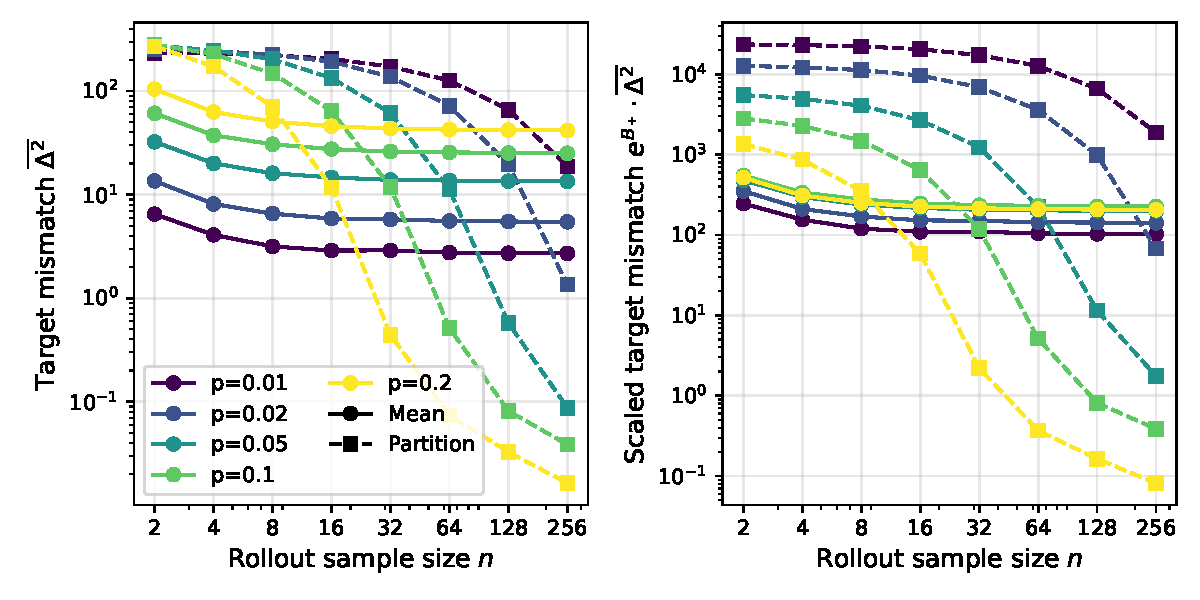
\includegraphics[width=0.75\columnwidth]{figs/compare_mean_partition_error_scaled_0.05.pdf}}
    \vspace{-0.1in}
    \caption{
      目标估计误差在 $\tau=0.05$  和 $p_t$  值域范围内从 $0.01$  到 $0.2$ 。  
左图：目标估计误差 $\overline{\Delta^2}$ 。右图：对应预因子 $e^{B_+}$  的缩放估计误差在 \eqref{eq:one_step_improvement}。该图展示了从 $100$  个随机种子的平均结果。  
当滚动样本大小 $n$  较小时，\textsc{PMD-part}\ 在小 $p_t$  时的误差要大得多。 
    }
    \label{fig:target_estimation}
    \end{center}
    \vspace{-0.15in}
\end{figure}

\subsubsection{对 \textsc{PMD-mean} 的精细化分析}
尽管理想目标与 \textsc{PMD-mean}\ 的估计目标之间的差距在 $n\to\infty$ 时并未消失，但经验损失 \eqref{eq:empirical-loss} 的最小化器在此极限下仍能恢复理想的目標策略，因为约束 $\mathbb{E}_{\pi_t}[e^{s_\pi}]=1$ 将对数比率从精确拟合优势值中拉回。  
在该大 $n$  regime 下，\Cref{prop:tgt_err_clean} 过于悲观。  
我们提供了更精细的分析，消除了误差下界。 
\begin{lemma}[Refined analysis for \pmdmean]\label{lem:pmdmean_refined}
    假设 \Cref{asm:realizable_plugin,asm:opt_err,asm:bounded_logratio,asm:finite_class} 成立，$r(y)\in\{0,1\}$ 且定义 $p_t\coloneqq \E_{y\sim\pi_t}[r(y)]$。  
令 $\varepsilon_n(p_t,\delta)$ 如 \Cref{prop:tgt_err_clean} 中所述。  
则对于任意 $\delta\in(0,1)$ ，以至少 $1-\delta$ 的概率，经验 \textsc{PMD-mean} 产生 $\widehat{\pi}_{t+1}$，使得 
    \begin{align*}
        \mathcal{L}_t(\widehat{\pi}_{t+1})
        \lesssim
        \frac{\log(\abs{\Pi}/\delta)}{\tau^2n} +\epsilon_{\mathrm{opt}} +\frac{p_t\cdot\varepsilon_n(p_t,\delta) + \varepsilon_n(p_t,\delta)^2}{\tau^2}.
    \end{align*}
\end{lemma}
完整的证明见附录~\ref{sec:refined}。  
\Cref{lem:pmdmean_refined} 表明 \textsc{PMD-mean}\ 现在与 \textsc{PMD-part}\ 在 \eqref{eq:erm_master_bound}(as $B_t^\mathrm{part}=O\bigl(\frac{1}{\tau}\bigr)$) 中具有相同的 $O\bigl(\frac{\log(\abs{\Pi}/\delta)}{\tau^2n}\bigr)$ 项，而 $\overline{\Delta^2}$ 项现在变为 $O\bigl(\frac{p_t}{\tau^2}\sqrt{\frac{p_t}{n}}+\frac{1}{\tau^2n^2}\bigr)$，当 $n\to \infty$ 时该项消失。  
这优于 \textsc{PMD-part}\ 在小 $n$ 且 $p_t$ 时的 $O\bigl(\frac{1}{\tau^2}\bigr)$ 误差。  
另一方面，当 $n=\Omega\bigl(\frac{1}{p_t}\bigr)$ 时，\textsc{PMD-part}\ 的误差为 $O(1)$，而 \textsc{PMD-mean}\ 的误差为 $O\bigl(\frac{p_t^2}{\tau^2}\bigr)$。  
这提示了 \textsc{PMD-mean}\ 的一种自适应正则化方案，即让 $\tau$ 随每个提示的通过率 $p_t$ 进行缩放，我们将其留待未来研究。 



\section{实验}
\label{sec:experiments}

我们在数学推理强化学习上进行实验，以验证 PMD 的实际性能。  
我们的实现基于 verl \citep{sheng2025hybridflow}。 

我们在 DAPO-Math-17k 数据集 \citep{yu2025dapo} 上使用基础模型 Qwen2.5-7B \citep{qwen2.5} 和 Qwen3-30B-A3B-Base \citep{yang2025qwen3} 进行训练。  
7B 模型训练了 495 个全局步骤（15 轮次），而 30B 模型则训练了 $300$ 个全局步骤。  
我们采用与 \citet{yu2025dapo} 相同的提示格式。  
奖励仅基于答案正确性，为二元 $\pm 1$。 

我们将全局批量大小设置为 512 个提示，组大小为 16，回滚时的采样温度为 1。  
Qwen2.5-7B 的最大响应长度为 8192，Qwen3-30B-A3B-Base 的最大响应长度为 20480。  
我们使用 32 个提示（512 个序列）的小批量进行训练，学习率 $1\times 10^{-6}$。

我们在 AIME 2024 和 AIME 2025 上进行评估。  
对于每个问题，我们采样 32 个解，并报告平均得分。  
我们主要使用 GRPO \citep{shao2024deepseekmath} 作为基准。  
为了效率对比，我们也包含同策略梯度方法，将全局批量大小（rollout 提示）设为 32，使其等于小批量大小。  
更多实现细节见 \Cref{sec:appendix-experiment}。 

\subsection{主要结果}
主要结果如 \Cref{tab:main-results} 所示。  
\textsc{PMD-mean} 显著优于 GRPO 基准：$\tau=0.005$ 在 7B 模型上分别实现 +2.6\% AIME24 和 +9.0\% AIME25 的绝对提升，$\tau=0.1$ 在 30B MoE 模型上分别实现 +14.6\% AIME24 和 +8.1\% AIME25 的绝对提升。 

\begin{table}[t]
    \caption{总体评估得分（Avg@32）。陈旧性表示使用同一旧策略进行回溯的最小步数数量。}
    \label{tab:main-results}
    \begin{center}\small
                \begin{tabular}{lcccc}
                \toprule
                \textbf{Method ($\tau$)} & \textbf{Staleness} & \textbf{AIME 24} & \textbf{AIME 25} & \textbf{Average} \\
                \midrule
                \multicolumn{5}{c}{\textbf{Qwen2.5-7B}} \\
                \midrule
                GRPO (-) & 16 & 17.08 & 10.52 & 13.80 \\
                On-policy (-) & 1 & 18.65 & \underline{18.33} & \underline{18.49} \\
                \pmdmean\ (0.005) & 16 & \underline{19.69} & \textbf{19.48} & \textbf{19.58} \\
                \pmdmean\ (0.01) & 16 & 17.60 & 17.50 & 17.55 \\
                \pmdmean\ (0.02) & 16 & \textbf{22.50} & 16.67 & \textbf{19.58} \\
                \midrule
                \multicolumn{5}{c}{\textbf{Qwen3-30B-A3B-Base}} \\
                \midrule
                GRPO (-) & 16 & 36.56 & 27.92 & 32.24 \\
                \pmdmean\ (0.01) & 16 & \underline{50.00} & \underline{35.10} & \underline{42.55} \\
                \pmdmean\ (0.1) & 16 & \textbf{50.83} & \textbf{37.19} & \textbf{44.01} \\
                \bottomrule
                \end{tabular}
    \end{center}
\end{table}

\begin{table}[tb]
    \caption{比较同策略梯度与\textsc{PMD-mean}的效率。计时单位为每token毫秒。尽管演员更新成本相当，但更大的全局批量大小（高过时）可分摊推理成本，从而减少整体训练时间。}
    \label{tab:efficiency_comparison}
    \begin{center}\small
                \begin{tabular}{lccc}
                \toprule
                \textbf{Method} & \textbf{Overall (ms/token)} & \textbf{Generation} & \textbf{Actor Update} \\
                \midrule
                On-policy & 0.0569 & 0.0512 & \textbf{0.0057} \\
                \pmdmean & \textbf{0.0126} & \textbf{0.0062} & 0.0064 \\
                \bottomrule
                \end{tabular}
    \end{center}
\end{table}

\textbf{更大全局批量大小带来的效率提升。}
如 \Cref{tab:main-results,tab:efficiency_comparison} 所示，相比于退化程度为 1 的同策略梯度，异策略 \textsc{PMD-mean}\ 通过利用更大的全局回溯批量大小，分摊了推理开销，实现了相当的性能表现，并获得了 $4.6\times$  的加速比。 


\textbf{稳定性。}
如图\Cref{fig:main_result}所示，\textsc{PMD-mean}\ 在训练过程中保持稳定，而\textsc{PMD-part}\ 则极不稳定，即使使用大得多的$\tau$仍可能崩溃。 

\begin{figure}[htb!]
    \vspace{-0.1in}
    \begin{center}

    \centerline{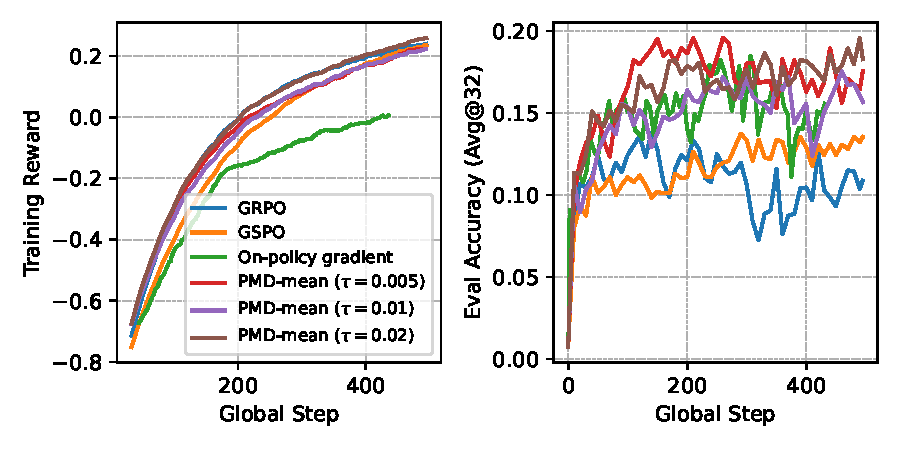
\includegraphics[width=0.5\columnwidth]{figs/fig5.pdf}
    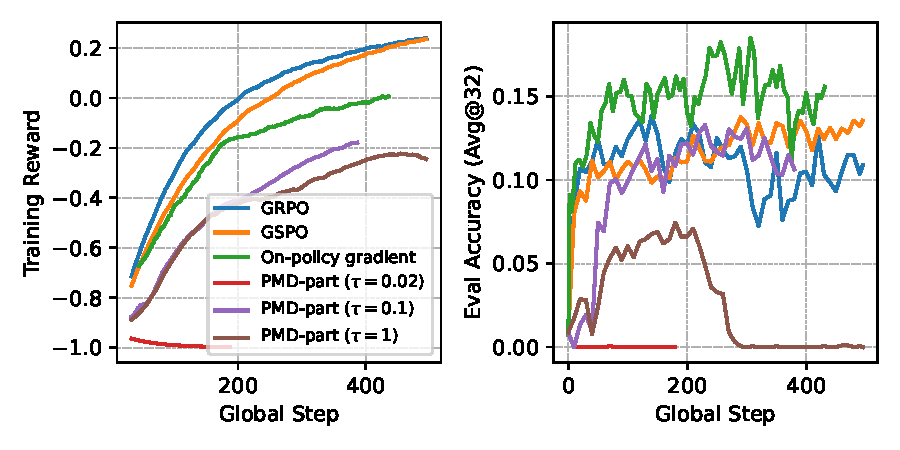
\includegraphics[width=0.5\columnwidth]{figs/fig6.pdf}}
    \caption{
        \textsc{PMD-mean}\ (上) 和 \textsc{PMD-part}\ (下) 的训练曲线（平滑后）及其在 DAPO-Math-17k 上 Qwen2.5-7B 的基准对比（左），以及在 AIME 2024 和 AIME 2025 上的平均评估准确率（右）。同策略策略梯度的全局步数除以 16 以与其他算法保持一致。 
    }
    \label{fig:main_result}
    \end{center}
    \vspace{-0.15in}
\end{figure}


\textbf{策略比率。}
我们记录了在上一个迷你步中的演员策略 $\pi_\theta$ 与该全局步的旧回放策略 $\pi_t$ 之间的对数策略比率，将其作为 $\log\frac{\pi_{t+1}}{\pi_t}$ 的近似值。
如 \Cref{fig:min_ratio} 所示，趋势验证了我们在 \Cref{sec:BB_instantiation} 中的理论，即 \textsc{PMD-mean}\ 中的策略下降比 \textsc{PMD-part}\ 更弱，并且随着训练进行和准确率提升，其下降趋势变得更强。 

\begin{figure}[tb]
  \begin{center}
    \centerline{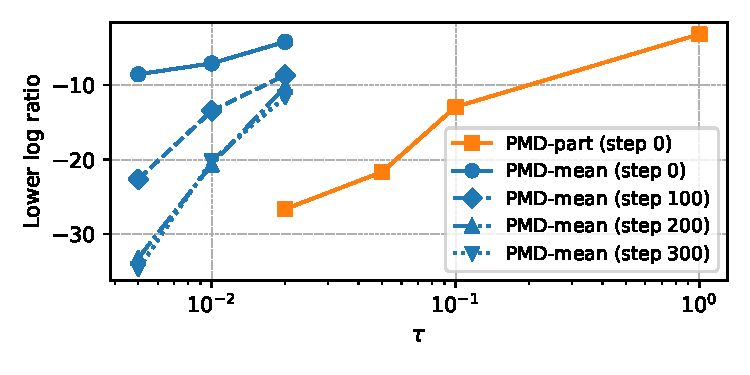
\includegraphics[width=0.6\columnwidth]{figs/fig7_ratio_scatter.pdf}}
    \vspace{-0.15in}
    \caption{
        \textsc{PMD-mean} 和 \textsc{PMD-part} 中对数比率的极小点 $\log\frac{\pi_{t+1}}{\pi_t}$，从最后一次更新的批量中估计得到。 
    }
    \label{fig:min_ratio}
  \end{center}
  \vspace{-0.25in}
\end{figure}

\textbf{超越标准GRPO。} 
标准GRPO在训练大型MoE模型时面临稳定性问题。 
我们进一步将 \textsc{PMD-mean}\ 与GSPO \citep{zheng2025group} 进行比较，后者是GRPO的一种先进变体，通过引入序列级重要性采样（IS）并结合截断和几何平均规范化来解决这一MoE稳定性问题，从而在性能上优于GRPO。 
结果如 \Cref{tab:gspo} 所示。 
如图所示，\textsc{PMD-mean}\ 在Qwen2.5-7B上表现优于GSPO，并在Qwen3-30B-A3B-Base MoE模型上达到了相当的性能。 
更多详细结果见 \Cref{sec:appendix-experiments-supp}。 


\begin{table}[htb!]
    \caption{\textsc{PMD-mean} 与 GSPO（Avg@32）的比较。 }
    \label{tab:gspo}
    \begin{center}\small
                \begin{tabular}{lcccc}
                \toprule
                \textbf{Method} & \textbf{Model} & \textbf{AIME 24} & \textbf{AIME 25} & \textbf{Average} \\
                \midrule
                GSPO & 7B & 15.52 & 11.98 & 13.75 \\
                \pmdmean\ & 7B & \textbf{19.69} & \textbf{19.48} & \textbf{19.58} \\
                \midrule
                GSPO & 30B & \textbf{53.33} & 34.58 & {43.96} \\
                \pmdmean\ & 30B & {50.83} & \textbf{37.19} & \textbf{44.01} \\
                \bottomrule
                \end{tabular}
    \end{center}
\end{table}

\section{相关工作}
\label{sec:related}

\textbf{大模型后训练中的强化学习。}
当前大模型后训练与对齐框架主要采用基于人类或人工智能反馈的强化学习（RLHF/RLAIF，\citealt{ziegler2019fine,ouyang2022training,bai2022constitutional}）或可验证奖励（RLVR，\citealt{lambert2024tulu}）。
该范式在数学推理、编程和逻辑任务方面展现出显著成效，进而推动了大规模强化学习方法及面向日益复杂智能体能力的架构设计发展 \citep{jaech2024openai,guo2025deepseek,google2025gemini,team2025kimik20}。

策略梯度方法 \citep{williams1992simple,sutton1999policy}，特别是 TRPO 和 PPO \citep{schulman2015trust,schulman2017proximal}，已在强化学习中确立了基础性地位。  
然而，在大语言模型后训练的背景下，维持参数化的价值网络（评论员模型）会引入显著的估计偏差和计算开销。  
为缓解这些局限性，近期的方法如 GRPO \citep{shao2024deepseekmath} 和 RLOO \citep{ahmadian2024back} 去除了评论员组件，转而利用从每个提示的多个蒙特卡罗样本中估计的基于组别的相对基准。  
更先进的方法，如 DAPO \citep{yu2025dapo}，通过高级最优化技术进一步提升了性能。

这些方法在本质上依赖于与当前策略分布高度匹配的采样分布，因此需要异策略修正机制以维持训练稳定性。  
尽管PPO/GRPO在token层面实现带裁剪的重要性采样（IS），但更近期的算法如GSPO \citep{zheng2025group}和CISPO \citep{chen2025minimax}采用序列级重要性采样或分离式裁剪重要性采样，以在训练混合专家（MoE）模型时提升稳定性。  
另有研究从基础设施层面解决训练-推理分布不匹配问题，提出了包括截断重要性采样 \citep{yao2025offpolicy} 和掩码重要性采样 \citep{liu-li-2025-rl-collapse} 在内的方法论改进。  
尽管这些技术部分有效，但显著增加了算法复杂度，并引入了大量难以进行理论分析的经验性调整。  
相比之下，我们的研究聚焦于一种极简的PMD算法，该算法在保持良好经验性能的同时，提供了更高的可分析透明性。


\textbf{策略镜像下降}

镜像下降框架 \citep{nemirovski1983problem} 为强化学习 \citep{geist2019theory,tomarmirror} 中的策略最优化提供了经典表述，其中大量文献分析了其理论迭代和样本复杂度 \citep{xiao2022convergence,zhan2023policy,lan2023policy,yuan2023linear,alfano2023novel,xu2024sample}。

然而，这些分析主要针对表格型情景或具有丰富样本的函数逼近情景，而非大语言模型后训练中rollouts必然受限的实际约束。

我们的工作建立了实际大语言模型后训练方法与Bregman散度选择之间的新联系，表明\textsc{PMD-mean}隐式地优化了一种自适应混合KL-$\chi^2$正则化项。

这种混合正则化方法与 $\chi^2$ PO \citep{huang2024correcting} 具有概念上的相似性，后者采用混合KL-$\chi^2$散度以减轻分布偏移条件下KL正则化DPO \citep{rafailov2023direct}中的过拟合。

尽管其他正则化方案已在离线偏好学习情景 \citep{wang2023beyond} 中被研究，我们的研究专门解决在线策略最优化的挑战。

文献提供了多种基于回归的方法来近似 \textsc{PMD-part} 中理想的KL解。  
\citet{richemond2024offline} 提出引入一个价值网络来估计对数配分函数，这一思路可追溯至 \citet{nachum2017bridging}。  
\citet{gao2024rebel} 开发了一种拟合成对相对奖励的技术，彻底消除了配分项。  
\citet{bartoldson2025trajectory} 在损失中使用其余所有项的组平均值（带停止梯度）来近似对数配分项。  
相比之下，\textsc{PMD-mean}\ \citep{team2025kimik15} 采用更简单的策略，直接用平均奖励来近似对数配分函数。  
我们的分析重点在于刻画这一实用近似的理论性质，并建立其数学基础。

\section{结论}
\label{sec:conclusion}
本文对 \textsc{PMD-mean} 进行了全面分析，该算法是一种在领先语言模型中已部署的大规模语言模型后训练实用算法。  
分析通过Lambert-$W$ 函数对算法的总体更新进行了确切刻画，建立了其与求解带有自适应混合KL--$\chi^2$ 正则化项的镜面下降子问题的数学等价性。  
这一理论框架揭示了该算法稳定性的具体机制：所诱导的 $\chi^2$ 项系统性地约束了大概率比的变化，有效防止了过度激进的策略更新，从而避免了训练不稳定的问题。

本研究刻意聚焦于 \textsc{PMD-mean}\ 的原则性形式，以实现更清晰的理论分析与理解。  
诸如过采样策略和重要性采样校正等先进技术，可用于解决训练/推理引擎不匹配问题，有望进一步提升 \textsc{PMD-mean}\ 的性能，这些方向将留待未来研究。  
通过阐明 \textsc{PMD-mean}\ 的基本数学性质，本文工作有助于推动面向大语言模型后训练的、具有理论基础且实际有效的强化学习算法的发展，可能实现更简单、更鲁棒且可扩展的方法，应对这一日益关键的任务。




\bibliography{ref}
\bibliographystyle{bibstyle}

\newpage
\appendix
\onecolumn

\section{实验细节}
\label{sec:appendix-experiment}
我们基于DAPO-Math-17k进行训练\footnote{\url{https://huggingface.co/datasets/BytedTsinghua-SIA/DAPO-Math-17k}} 数据集（去重后）。  
基础模型包括 Qwen2.5-7B\footnote{\url{https://huggingface.co/Qwen/Qwen2.5-7B}} 和 Qwen3-30B-A3B-Base\footnote{\url{https://huggingface.co/Qwen/Qwen3-30B-A3B-Base}}. 

\subsection{提示模板}
我们的提示模板遵循 \citet{yu2025dapo}，所有问题 \texttt{problem\_statement} 均按以下形式处理。 
\begin{tcblisting}{listing only, title=Chain-of-Thought (CoT) Prompt Template}
Solve the following math problem step by step. The last line of your response should be of the form Answer: $Answer (without quotes) where $Answer is the answer to the problem.

{problem_statement}

Remember to put your answer on its own line after "Answer:".
\end{tcblisting}

\subsection{超参数}
我们总结了 \Cref{tab:hyperparams} 中的关键超参数。 
\begin{table}[htb]
    \centering
    \caption{7B稠密模型和30B MoE模型实验的关键超参数。}
    \label{tab:hyperparams}
    \small
    \begin{tabular}{lcc}
        \toprule
        \textbf{Parameter} & \textbf{7B Dense} & \textbf{30B MoE} \\
        \midrule
        trainer.nnodes & 4 & 8 \\
        trainer.n\_gpus\_per\_node & 8 & 8 \\
        distributed strategy & FSDP & Megatron \\
        model.path & Qwen/Qwen2.5-7B & Qwen/Qwen3-30B-A3B-Base \\
        \midrule
        data.train\_batch\_size (prompts) & 512 & 512 \\
        data.gen\_batch\_size (prompts) & 512 & 512 \\
        data.max\_prompt\_length & 2048 & 2048 \\
        data.max\_response\_length & 8192 & 20480 \\
        \midrule
        rollout.name & vLLM & vLLM \\
        rollout.n (group size) & 16 & 16 \\
        rollout.temperature & 1.0 & 1.0 \\
        rollout.top\_p & 1.0 & 1.0 \\
        rollout.max\_model\_len & 10240 & 22528 \\
        val\_kwargs.n (avg@k) & 32 & 32 \\
        val\_kwargs.temperature & 1.0 & 1.0 \\
        val\_kwargs.top\_p & 0.7 & 0.7 \\
        \midrule
        actor.ppo\_epochs & 1 & 1 \\
        actor.ppo\_mini\_batch\_size (prompts) & 32 & 32 \\
        actor.clip\_ratio\_low / high (GRPO) & 0.2 / 0.2 & 0.2 / 0.2 \\
        actor.clip\_ratio\_low / high (GSPO) & 3e-4 / 4e-4 & 3e-4 / 4e-4 \\
        optim.lr & 1e-6 & 1e-6 \\
        optim.betas & [0.9, 0.999] & [0.9, 0.999] \\
        optim.weight\_decay & 0.01 & 0.01 \\
        grad clip & 1.0 & 1.0 \\
        \midrule
        tensor\_model\_parallel\_size & 1 & 2 \\
        pipeline\_model\_parallel\_size & 1 & 2 \\
        expert\_model\_parallel\_size & N/A & 8 \\
        \bottomrule
    \end{tabular}
\end{table}


\subsection{实现细节}
我们的实现基于verl\footnote{\url{https://github.com/verl-project/verl}} \citep{sheng2025hybridflow}. 
对于 GRPO 和 GSPO，我们遵循 DAPO 的方法，禁用相对于基础参考模型的显式 KL 惩罚 \citep{yu2025dapo}。  
对于每个提示 $x$，我们从旧策略 $\pi_t(\cdot\mid x)\coloneqq\pi_{\theta_t}(\cdot\mid x)$ 中采样 $K$ 个响应 $y_1,\dots,y_K\sim \pi_t(\cdot\mid x)$，并根据答案的正确性获得奖励 $r_i\coloneqq r(x,y_i)\in\{-1,+1\}$。  
设 $\pi_\theta$ 为可训练策略，我们有 $\log \pi_\theta(y\mid x)= \sum_{j=1}^{\abs{y}}\log \pi_\theta(y_j\mid x,y_{<j})$。 

定义token概率比和几何规范化序列概率比如下： 
\begin{align*}
    \rho_{i,j}(\theta)\coloneqq \frac{\pi_\theta(y_{i,j}\mid x,y_{i,<j})}{\pi_t(y_{i,j}\mid x,y_{i,<j})}, 
    \quad
    s_{i}(\theta)\coloneqq \left(\frac{\pi_\theta(y_i\mid x)}{\pi_t(y_i\mid x)}\right)^{\frac{1}{\abs{y_i}}}. 
\end{align*}
此外，定义以下优点： 
\begin{align*}
    \widehat{A}^{\mathrm{grpo}}_i\coloneqq \frac{r_i-\mathrm{mean}(r_1,\dots,r_K)}{\mathrm{std}(r_1,\dots,r_K)}, 
    \quad
    \widehat{A}^{\mathrm{loo}}_i\coloneqq r_i-\frac{1}{K-1}\sum_{j\neq i} r_j,
    \quad
    \widehat{A}^{\mathrm{part}}_i\coloneqq r_i-\tau\log\left(\frac{1}{K-1}\sum_{j\neq i} e^{r_j/\tau}\right).
\end{align*}

GRPO \citep{shao2024deepseekmath} 损失定义为
\begin{align*}
    \mathcal{L}_\mathrm{GRPO}(\theta)=
    -\mathbb{E}_{x\sim \mathcal{D}}\mathbb{E}_{y_1,\dots,y_K\sim\pi_t(\cdot\mid x)}\left[\frac{1}{K}\sum_{i=1}^K\frac{1}{\abs{y_i}}\sum_{j=1}^{\abs{y_i}} \min\Big(\rho_{i,j}(\theta)\widehat{A}^{\mathrm{grpo}}_i, \mathrm{clip}(\rho_{i,j}(\theta),1-\epsilon,1+\epsilon)\widehat{A}^{\mathrm{grpo}}_i\Big)\right],
\end{align*}
其中 $\epsilon=0.2$，我们舍弃了 KL 罚项。 

当全局批量大小设置为与小批量大小相同时，GRPO退化为带有优势估计量的同策略梯度 $\widehat{A}^\mathrm{grpo}_i$。  
经验上，我们发现使用 $\widehat{A}^\mathrm{loo}_i$ 可获得相似的性能，因此在同策略梯度实验中我们采用（长度规范化的）RLOO \citep{ahmadian2024back} 损失。 
\begin{align*}
    \mathcal{L}_{\mathrm{RLOO}}(\theta) = -\mathbb{E}_{x\sim \mathcal{D}}\mathbb{E}_{y_1,\dots,y_K\sim\pi_t(\cdot\mid x)} \left[\frac{1}{K}\sum_{i=1}^K\frac{1}{\abs{y_i}}\widehat{A}^{\mathrm{loo}}_i \log \pi_\theta(y_i\mid x)\right].
\end{align*}

GSPO \citep{zheng2025group} 损失定义如下： 
\begin{align*}
    \mathcal{L}_{\mathrm{GSPO}}(\theta) = -\mathbb{E}_{x\sim \mathcal{D}}\mathbb{E}_{y_1,\dots,y_K\sim\pi_t(\cdot\mid x)}\left[\frac{1}{K}\sum_{i=1}^K \min\Big(s_{i}(\theta)\widehat{A}^{\mathrm{grpo}}_i, \mathrm{clip}(s_i(\theta),1-\epsilon_\mathrm{low},1+\epsilon_\mathrm{high})\widehat{A}^{\mathrm{grpo}}_i\Big)\right],
\end{align*}
其中 $\epsilon_\mathrm{low}=3\times 10^{-4}$ 和 $\epsilon_\mathrm{high}=4\times 10^{-4}$ 如所建议。 

我们实现了 \textsc{PMD-mean}\ \citep{team2025kimik15} 和 \textsc{PMD-part} 使用以下损失。 
\begin{align*}
    \mathcal{L}_{\mathrm{mean}}(\theta) = \mathbb{E}_{x\sim \mathcal{D}}\mathbb{E}_{y_1,\dots,y_K\sim\pi_t(\cdot\mid x)} \left[\frac{1}{K}\sum_{i=1}^K\frac{\tau}{\abs{y_i}}\left(\log\frac{\pi_\theta(y_i\mid x)}{\pi_t(y_i\mid x)}-\frac{\widehat{A}^{\mathrm{loo}}_i}{\tau}\right)^2 \right],\\
    \mathcal{L}_{\mathrm{part}}(\theta) = \mathbb{E}_{x\sim \mathcal{D}}\mathbb{E}_{y_1,\dots,y_K\sim\pi_t(\cdot\mid x)} \left[\frac{1}{K}\sum_{i=1}^K\frac{\tau}{\abs{y_i}}\left(\log\frac{\pi_\theta(y_i\mid x)}{\pi_t(y_i\mid x)}-\frac{\widehat{A}^{\mathrm{part}}_i}{\tau}\right)^2 \right].
\end{align*}
在损失函数中的因子 $\tau$ 保证了在调整 $\tau$ 时梯度范数不会相差过大，且长度规范化与其他方法中的损失聚合模式保持一致。 

\subsection{补充结果}\label{sec:appendix-experiments-supp}
我们在 \Cref{fig:results-7B,fig:results-30B} 中提供了补充的实验结果。 

\begin{figure}[ht]
  \begin{center}
    \centerline{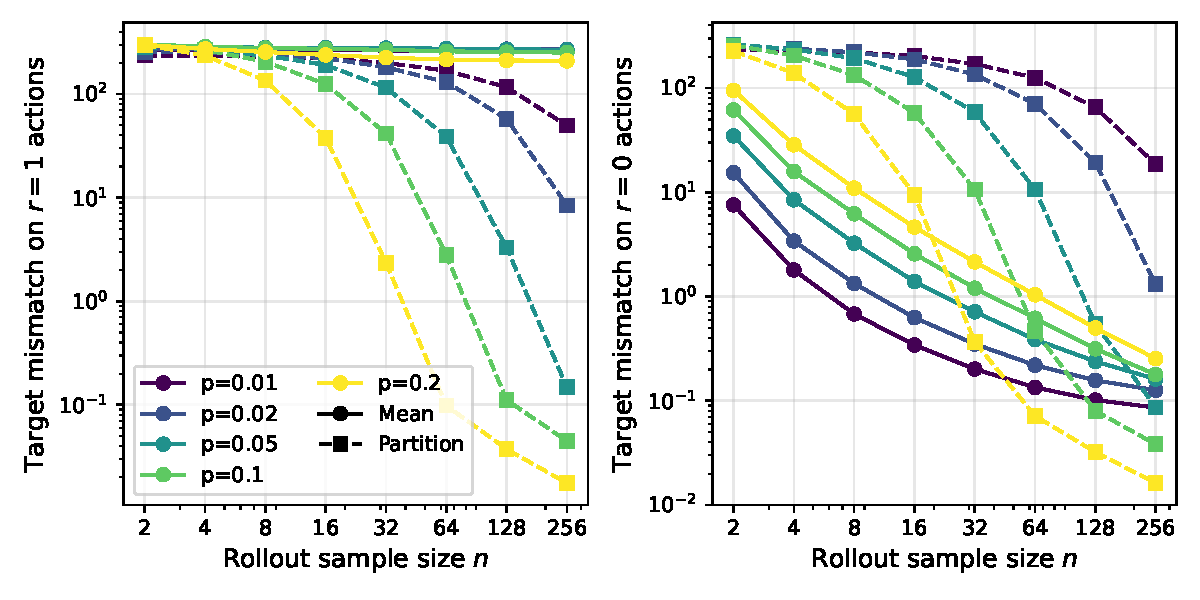
\includegraphics[width=0.75\columnwidth]{figs/compare_mean_partition_error_actions_0.05.pdf}}
    \caption{
      \textsc{PMD-mean}\ 和 \textsc{PMD-part}\ 在 $\tau=0.05$  和 $p_t$  值域范围内，针对正负动作的 目标估计误差 从 $0.01$  到 $0.2$ 。  
左图：正动作。右图：负动作。  
该图展示了从 $100$  个随机种子得到的平均值。  
\textsc{PMD-mean}\ 中的误差主要来源于正目标之间的系统性不匹配。 
    }
    \label{fig:target_actions}
  \end{center}
\end{figure}

\begin{figure}[ht]
  \begin{center}
    \centerline{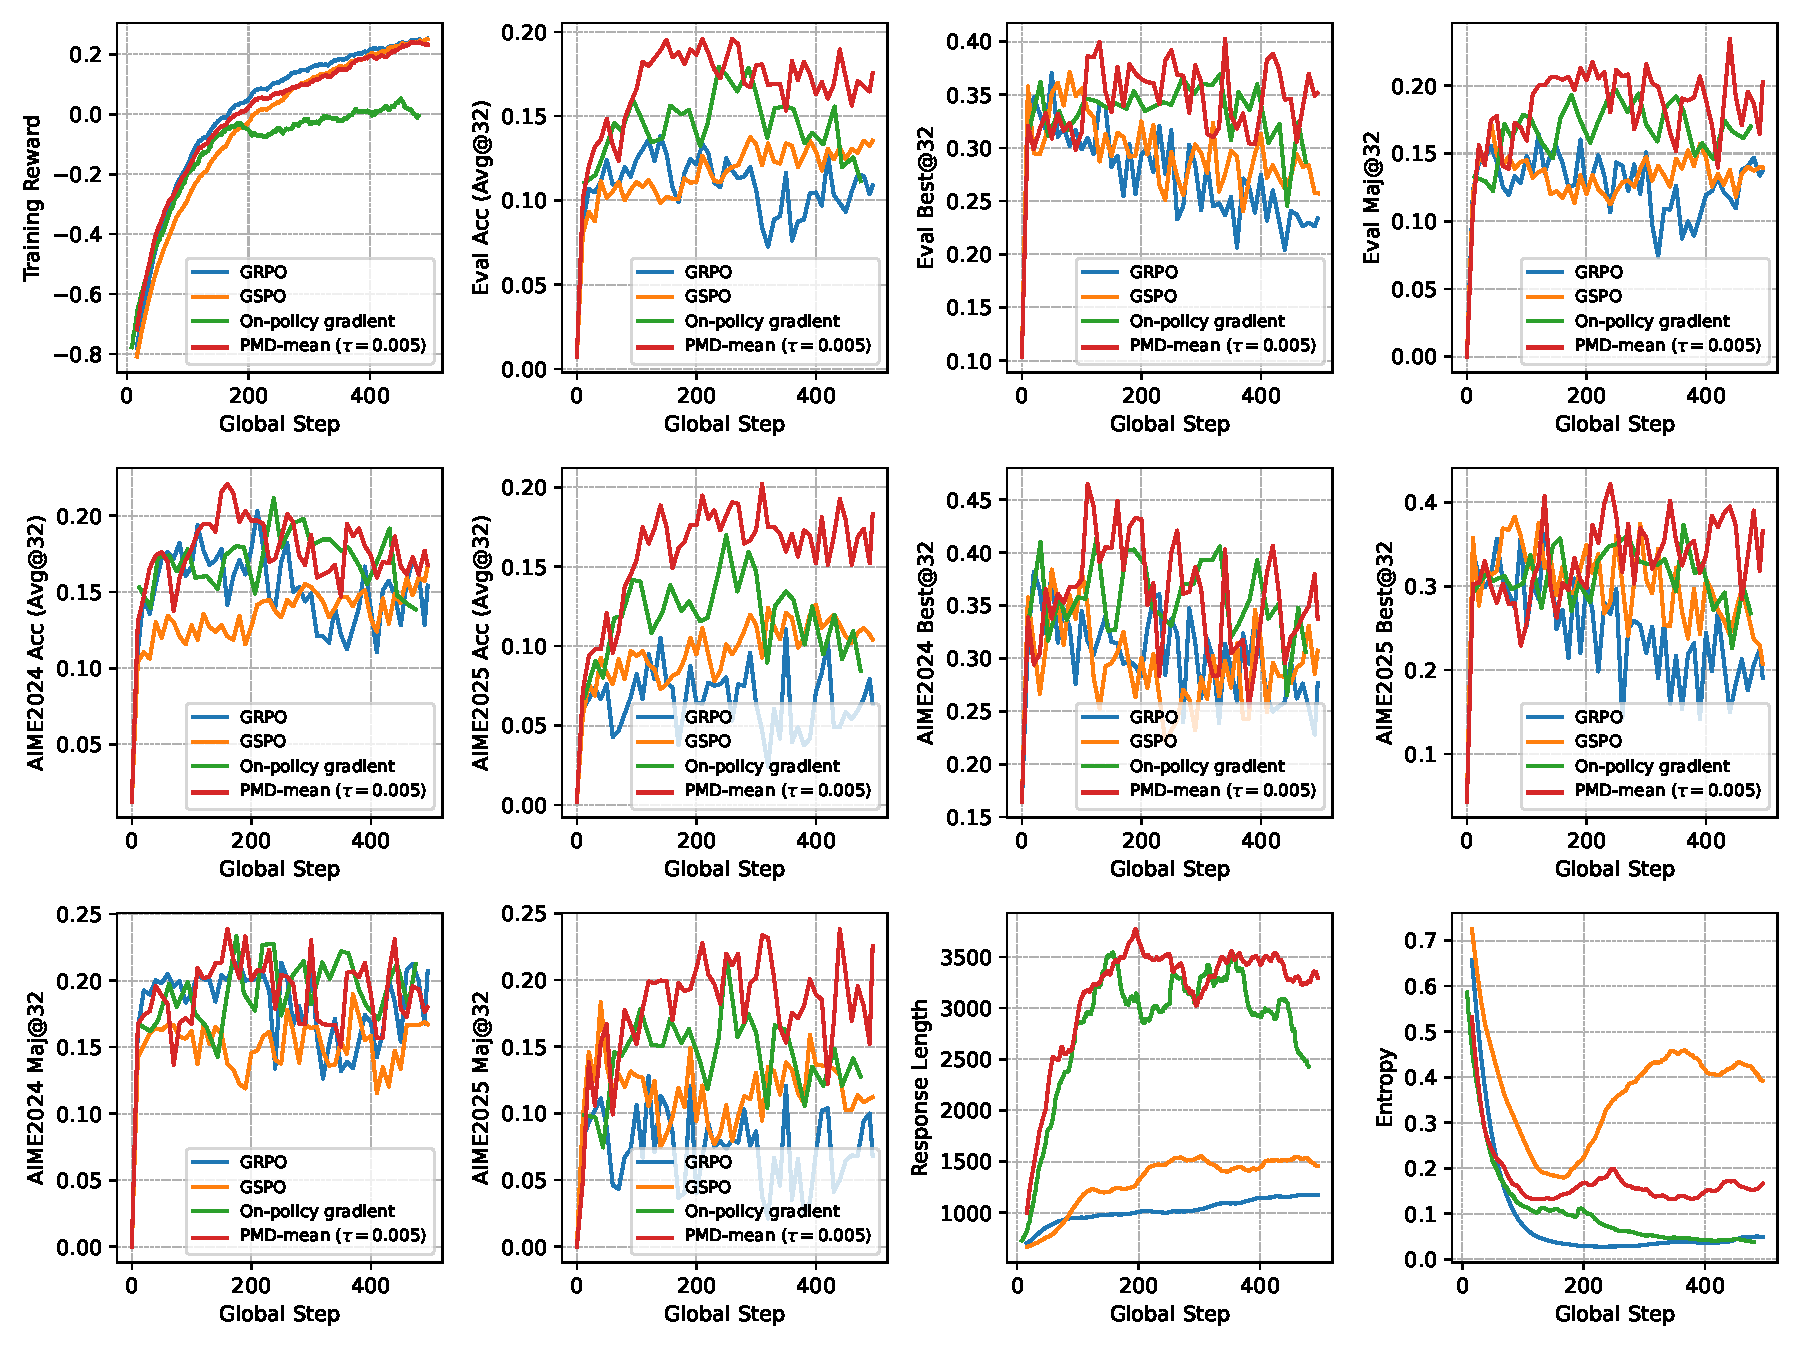
\includegraphics[width=\columnwidth]{figs/fig10_large.pdf}}
    \caption{
      Qwen2.5-7B 在 15 轮次（495 个全局步骤）下的训练结果。训练奖励、响应长度和熵通过指数移动平均（EMA）平滑，有效窗口大小为 50。  
      \textsc{PMD-mean}\ 在 Pass@1（以 Avg@32 衡量）以及 Pass@32 和 Maj@32（绝对多数投票答案的准确率）方面均表现出更优性能。 
    }
    \label{fig:results-7B}
  \end{center}
\end{figure}

\begin{figure}[ht]
  \begin{center}
    \centerline{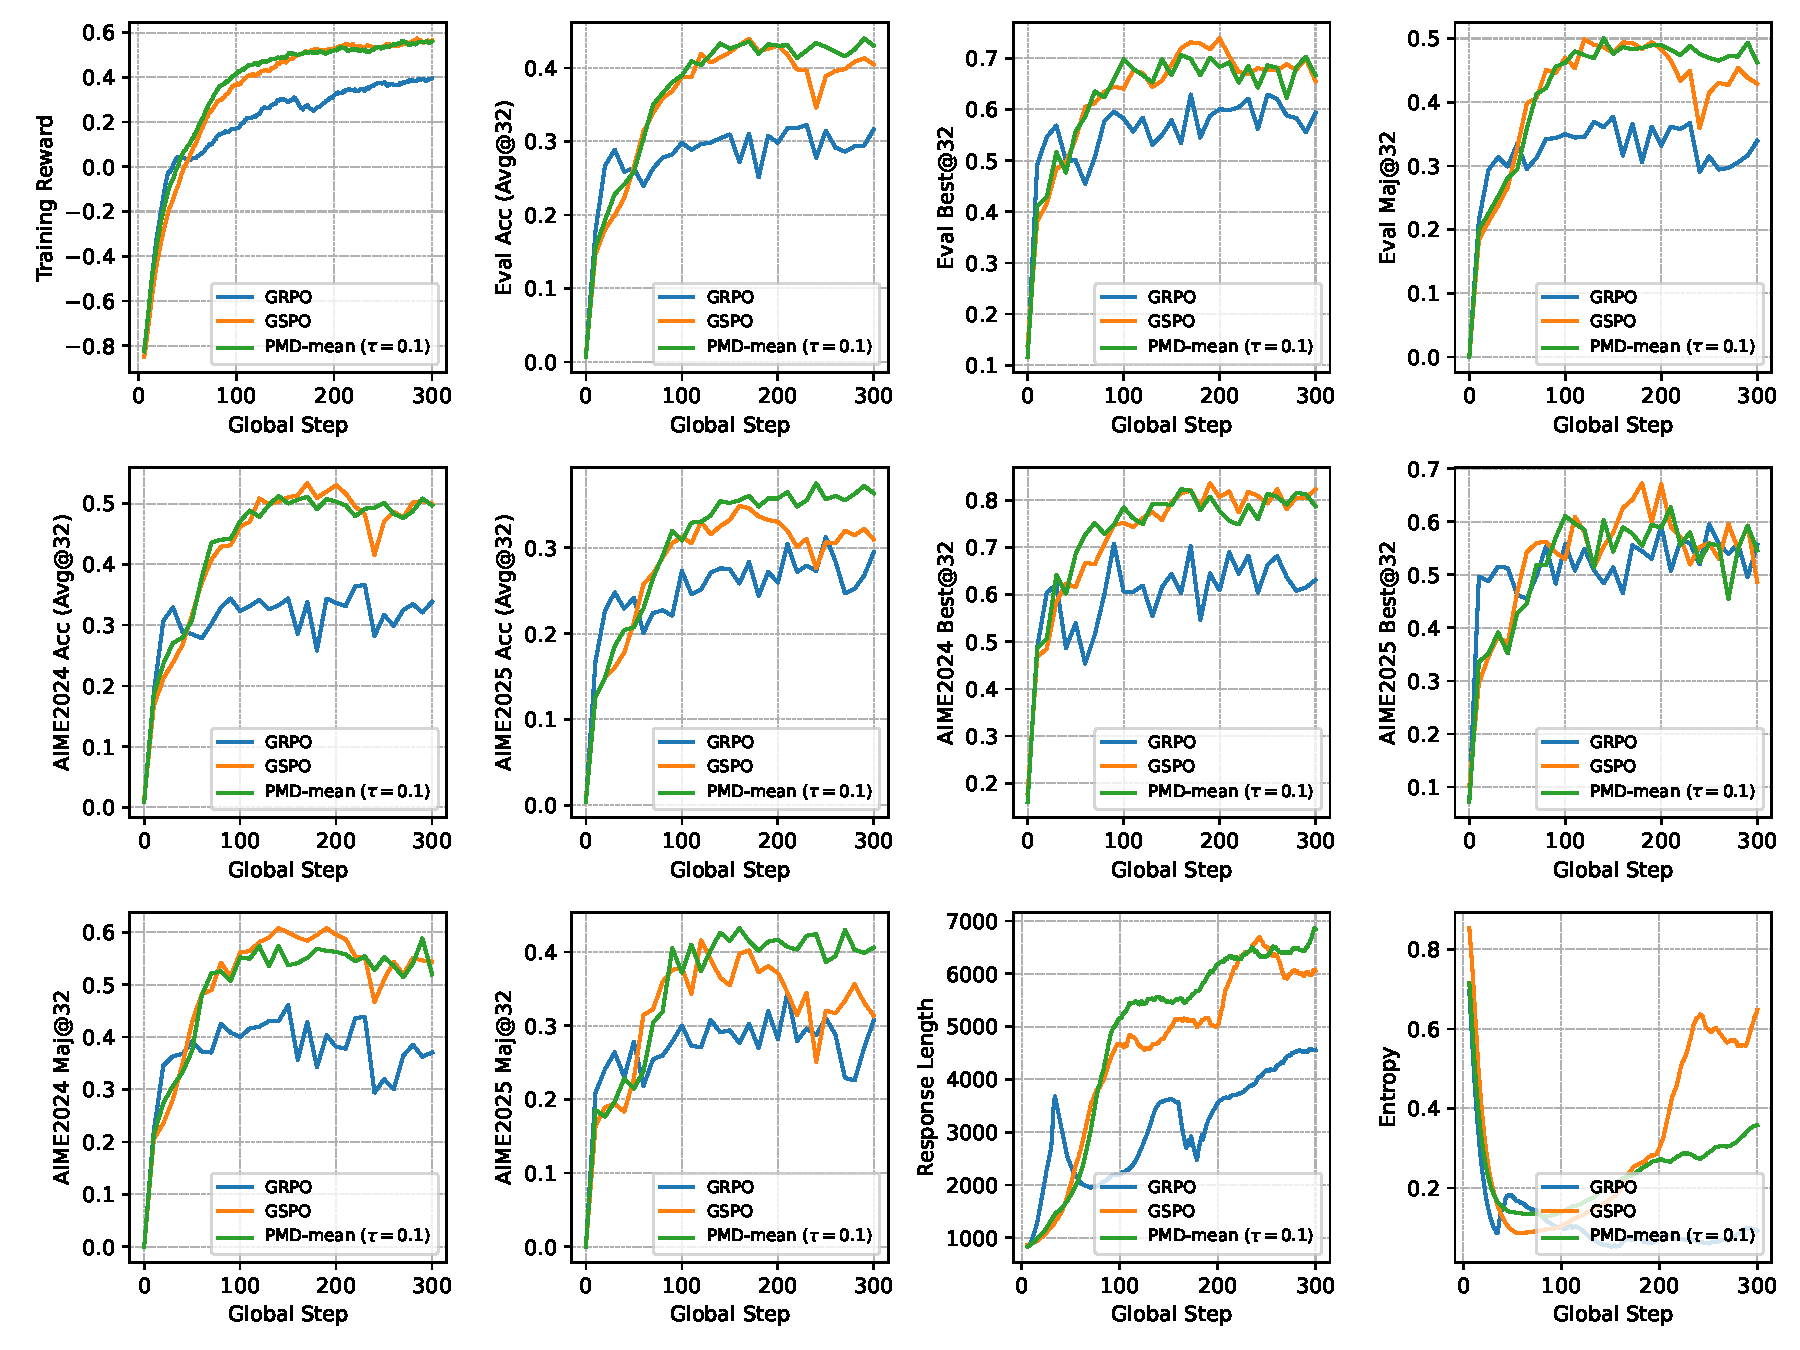
\includegraphics[width=\columnwidth]{figs/fig9_large.pdf}}
    \caption{
      Qwen3-30B-A3B-Base 在 300 个全局步骤下的训练结果。训练奖励、响应长度和熵通过指数移动平均（EMA）进行平滑处理，有效窗口大小为 20。 
    }
    \label{fig:results-30B}
  \end{center}
\end{figure}

\section{第~\ref{sec:pmdmean}~节中缺失的证明}
\subsection{证明 \Cref{thm:pmdmean_solution}}
\label{sec:proof_thm1}
\begin{proof}[Proof of Theorem~\ref{thm:pmdmean_solution}]
    定义 $u(y)=\log\frac{\pi(y)}{\pi_t(y)}$ ，则 $\mathcal{L}_{\mathrm{mean}}$  （在策略空间中）的拉格朗日量可表示为
    \begin{align*}
        L(u,\lambda)=\frac{1}{2}\sum_{y\in\mathcal{Y}}\pi_t(y)(\Delta_y-\tau u(y))^2 + \lambda\cdot\left(\sum_{y\in\mathcal{Y}}\pi_t(y)e^{u(y)}-1\right),
    \end{align*}
    KKT条件给出 
    \begin{align*}
        \begin{cases}-\tau\pi_t(y)(\Delta_y-\tau u(y)) + \lambda\pi_t(y)e^{u(y)}=0,~\forall y\in\mathcal{Y},\\
        \sum_{y\in\mathcal{Y}}\pi_t(y)e^{u(y)}=1.
        \end{cases}
    \end{align*}
    假设对所有 $y\in\mathcal{Y}$  均有 $\pi_t(y)>0$（这对没有 top-p/top-k 约束的大模型是成立的），则 $\mathcal{L}_{\mathrm{mean}}$  的任意驻点都应满足 
    \begin{align}
        -\tau(\Delta_y-\tau u(y))+\lambda e^{u(y)}=0
        &\iff \tau(\Delta_y-\tau u(y))e^{-u(y)}=\lambda\notag\\
        &\iff \left(\frac{\Delta_y}{\tau}-u(y)\right)e^{\frac{\Delta_y}{\tau}-u(y)}=\frac{\lambda}{\tau^2}e^{\frac{\Delta_y}{\tau}}\notag\\
        &\iff \frac{\Delta_y}{\tau}-u(y)=W\left(\frac{\lambda}{\tau^2}e^{\frac{\Delta_y}{\tau}}\right)\notag\\
        &\iff u(y)=\frac{\Delta_y}{\tau}-W\left(\frac{\lambda}{\tau^2}e^{\frac{\Delta_y}{\tau}}\right).\label{eq:KKT-mean}
    \end{align}
    \eqref{eq:KKT-mean} 的右端关于 $\lambda$ 单调递减，且当 $\lambda=0$ 时关于 $\mathbb{E}_{\pi_t}[\text{RHS}]=0$ 单调递减。此外，根据 Jensen 不等式， 
    \begin{align*}
    1=\mathbb{E}_{y\sim\pi_t}[e^{u(y)}]\geq e^{\mathbb{E}_{y\sim\pi_t}[u(y)]}\implies\mathbb{E}_{y\sim\pi_t}[u(y)]\leq 0,
    \end{align*}
    因此，必须存在唯一的 $\lambda\geq 0$（因而也有唯一的 $u$）使得KKT条件成立。此外，在假设 $\pi_t(y)>0$ 成立的情况下，$u$ 中拉格朗日函数的海森矩阵是正定的，因此该点确实是 $\mathcal{L}_{\mathrm{mean}}$ 的极小化点。 

    为了刻画 $\lambda$ ，我们利用 $W$ 在所有 $z\geq 0$ 下的若干性质：(1) $\cW(z)$ 为凹函数且单调递增；(2) $\cW(z)\geq\frac{z}{1+z}$ ；(3) $e^{\cW(z)}=\frac{z}{\cW(z)}$ 。  
此外，根据可行性约束，我们有 
    \begin{align*}
        1
        &=\sum_{y\in\mathcal{Y}}\pi_t(y)\frac{\exp\left(\frac{\Delta_y}{\tau}\right)}{\exp\left(W\left( \frac{\lambda}{\tau^2} \exp\left(\frac{\Delta_y}{\tau}\right)\right)\right)}\\
        &=\sum_{y\in\mathcal{Y}}\pi_t(y)\frac{\exp\left(\frac{\Delta_y}{\tau}\right)W\left(\frac{\lambda}{\tau^2} \exp\left(\frac{\Delta_y}{\tau}\right)\right)}{\frac{\lambda}{\tau^2} \exp\left(\frac{\Delta_y}{\tau}\right)}\\
        &=\frac{\tau^2}{\lambda}\mathbb{E}_{y\sim\pi_t}\left[W\left(\frac{\lambda}{\tau^2} \exp\left(\frac{\Delta_y}{\tau}\right)\right)\right].
    \end{align*}
    为方便起见，令 $x\coloneqq\lambda/\tau^2\geq 0$ ，$A\coloneqq\mathbb{E}_{\pi_t}[e^{\Delta_y/\tau}]$ ，$B\coloneqq\mathbb{E}_{\pi_t}[e^{2\Delta_y/\tau}]$ 。则目标是证明 
    \begin{align*}
        \frac{A(A-1)}{B}\leq x\leq\log A.
    \end{align*}

    对于上界，利用凹性及詹森不等式， 
    \begin{align*}
        x=\mathbb{E}_{\pi_t}[\cW(xe^{\Delta_y/\tau})]
        \leq \cW(\mathbb{E}[xe^{\Delta_y/\tau}])
        =\cW(xA).
    \end{align*}
    由于 $W$ 是递增的，上述不等式意味着 
    \begin{align*}
        xe^x\leq \cW(xA)e^{\cW(xA)}=xA\implies e^x\leq A\implies x\leq\log A,
    \end{align*}
    从而证明了上界。

   另一方面，由对 $\cW$ 的下界可得 
    \begin{align*}
        x&=\mathbb{E}_{\pi_t}[\cW(xe^{\Delta_y/\tau})]\\
        &\geq\mathbb{E}_{\pi_t}\left[\frac{xe^{\Delta_y/\tau}}{1+xe^{\Delta_y/\tau}}\right]\\
        &\geq
        \frac{\left(\mathbb{E}_{\pi_t}[xe^{\Delta_y/\tau}]\right)^2}{\mathbb{E}_{\pi_t}[xe^{\Delta_y/\tau}(1+xe^{\Delta_y/\tau})]}\\
        &=\frac{(xA)^2}{xA+x^2B},
    \end{align*}
    第二个不等式来自柯西-施瓦茨不等式。解该不等式即可得到下界。

    对于二元奖励 $r\in\{0,1\}$ 且 $p=\E_{\pi_t}[r(y)]$ ，我们有 $\E_{\pi_t}[\Delta_y^2]=\Var(r)=p(1-p)$ 以及
    \begin{align}\label{eq:expression-x}
        x=p \cW(xe^{(1-p)/\tau}) + (1-p)\cW(xe^{-p/\tau}).
    \end{align}
    当 $\tau\to\infty$ 较大时，我们有 
    \begin{align*}
        &A=\mathbb{E}_{\pi_t}\left[1+\frac{\Delta_y}{\tau} + \frac{\Delta_y^2}{2\tau^2} + O(\tau^{-3})\right]=1+\frac{p(1-p)}{2\tau^2} + O(\tau^{-3}),\\
        &B=\mathbb{E}_{\pi_t}\left[1+\frac{2\Delta_y}{\tau} + \frac{2\Delta_y^2}{\tau^2} + O(\tau^{-3})\right]=1+\frac{2p(1-p)}{\tau^2} + O(\tau^{-3}).
    \end{align*}
    因此，$x=\lambda/\tau^2$ 的下界给出
    \begin{align*}
        A(A-1)\leq xB
        &\implies\left(\frac{p(1-p)}{2\tau^2}\right)\left(1+ O(\tau^{-2})\right)\leq \left(1+O(\tau^{-2})\right)\frac{\lambda}{\tau^2}\\
        &\implies \frac{p(1-p)}{2}-O(\tau^{-1})\leq\lambda.
    \end{align*}
    另一方面，上界给出
    \begin{align*}
        \lambda
        &\leq\tau^2\log A\\
        &=\tau^2\log\left(1+\frac{p(1-p)}{2\tau^2}+O(\tau^{-3})\right)\\
        &\leq\tau^2\left(\frac{p(1-p)}{2\tau^2}+O(\tau^{-3})\right)\\
        &=\frac{p(1-p)}{2}+O(\tau^{-1}).
    \end{align*}
    将两个界结合起来，我们得到 $\lambda=\frac{1}{2}p(1-p)+O(\tau^{-1})$ 为 $\tau\to\infty$。 

    对于较小的 $\tau\to 0$ ，边界 \eqref{eq:lambda_bounds} 过于宽松。  
我们定义 $v=\frac{\lambda}{\tau}=\tau x$ 并证明 $v\to p(1-p)$ 。  
首先，Lambert-$W$ 函数满足 
    \begin{align*}
        \log z-\log\log z\leq \cW(z)\leq \log z
    \end{align*}
    对于 $z>e$。  
此外，对于 $z\geq 0$，$\cW(z)=\frac{z}{e^{\cW(z)}}\leq z$。  
由于 $e^{-p/\tau}$ 随着 $\tau^{-1}$ 的增长比任何多项式都更快地衰减，我们有 
    \begin{align*}
        0\leq (1-p)\tau \cW(xe^{-p/\tau})
        \leq (1-p)\tau xe^{-p/\tau}
        =(1-p)ve^{-p/\tau}\to 0.
    \end{align*}
    因此，\eqref{eq:expression-x} 中的第二项消失。  
对于剩下的主要项，令 $z_1=xe^{(1-p)/\tau}=\frac{v}{\tau}e^{(1-p)/\tau}$ ，则当 $\tau\to 0$ 时，$z_1\to\infty$ ，且 $\log z_1=\frac{1-p}{\tau}+\log\frac{v}{\tau}$ 。  
在这种情况下，我们对Lambert-$W$ 函数的估计给出 
    \begin{align*}
        \tau \cW(z_1)
        =(1-p) + o(1),
    \end{align*}
    从而 
    \begin{align*}
        v=\tau x
        =\tau\left(p \cW(z_1) + o(1)\right)
        =p(1-p) + o(1)
        \implies 
        \lambda=\tau p(1-p)(1+o(1)).
    \end{align*}
\end{proof}

\subsection{策略比率}\label{sec:appendix-ratio}
我们正式陈述 \textsc{PMD-mean}\ 和 \textsc{PMD-part}\ 在 \Cref{eq:ratio_pos_mean,eq:ratio_pos_part,eq:ratio_neg_mean,eq:ratio_neg_part} 中的策略比例，如下所述。 
\begin{proposition}[Binary-reward ratios for small $\tau$]
\label{prop:binary_ratios}
    假设 $r(y)\in\{0,1\}$ 且令 $p=\E_{\pi_t}[r(y)]\in(0,1)$ 。  
考虑比值 $\rho(y)\coloneqq\pi_{t+1}(y)/\pi_t(y)$ 。

    \noindent\textbf{\textsc{PMD-mean}.}
    如 $\tau\to 0$ 所示，对于任意 $y$ 且满足 $r(y)=1$ ，
    \begin{align*}
        \rho^{\mathrm{mean}}_+(y)
        =\frac{1}{p}-\frac{1-p}{p}e^{-p/\tau}(1+o(1)),
    \end{align*}
    并且对于任意满足 $r(y)=0$ 的 $y$ ，
    \begin{align*}
        \rho^{\mathrm{mean}}_-(y)=e^{-p/\tau}(1+o(1)).
    \end{align*}

    \noindent\textbf{\textsc{PMD-part}.}
    对于任意 $\tau>0$ ，划分更新满足
    \begin{align*}
        \rho^{\mathrm{part}}_+(y)=\frac{1}{p+(1-p)e^{-1/\tau}},
        \quad
        \rho^{\mathrm{part}}_-(y)=\frac{e^{-1/\tau}}{p+(1-p)e^{-1/\tau}},
    \end{align*}
    以及特别地作为 $\tau\to 0$ ，
    \begin{align*}
        \rho^{\mathrm{part}}_+(y)=\frac{1}{p}-\frac{1-p}{p^2}e^{-1/\tau}+O(e^{-2/\tau}),
        \quad
        \rho^{\mathrm{part}}_-(y)=\frac{1}{p}e^{-1/\tau}+O(e^{-2/\tau}).
    \end{align*}
\end{proposition}
\begin{proof}[Proof of \Cref{prop:binary_ratios}]
    始终令 $x\coloneqq\lambda/\tau^2$ 。
    对于 \textsc{PMD-mean}，从 Lambert-$W$ 形式 \eqref{eq:pmdmean_lambertW_form} 出发，并使用 $e^{-\cW(z)}=\cW(z)/z$ 将比值重写为
    \begin{align}\label{eq:ratio_W_form}
        \frac{\pi^{\mathrm{mean}}_{t+1}(y)}{\pi_t(y)}
        =\exp\Big(\frac{\Delta_y}{\tau}-\cW(xe^{\Delta_y/\tau})\Big)
        =\frac{1}{x}W\big(xe^{\Delta_y/\tau}\big).
    \end{align}
    在二分类情况下，当 $\Delta=1-p$ 时 $r=1$，当 $r=0$ 时 $\Delta=-p$，因此定义
    \begin{align*}
        \rho^{\mathrm{mean}}_+ \coloneqq \frac{1}{x}W\Big(xe^{(1-p)/\tau}\Big),
        \quad
        \rho^{\mathrm{mean}}_- \coloneqq \frac{1}{x}W\Big(xe^{-p/\tau}\Big),
    \end{align*}
    我们有规范化恒等式
    \begin{align}
        \label{eq:norm_binary}
        1=\sum_y\pi^{\mathrm{mean}}_{t+1}(y)=p\rho^{\mathrm{mean}}_+ + (1-p)\rho^{\mathrm{mean}}_-.
    \end{align}

    由 \eqref{eq:lambda_asymptotics}，$\lambda\sim \tau p(1-p)$ 作为 $\tau\to 0$，因此
    \begin{align*}
        x=\frac{\lambda}{\tau^2}\sim \frac{p(1-p)}{\tau}=\Theta\left(\frac{1}{\tau}\right).
    \end{align*}
    因此 $xe^{-p/\tau}\to 0$  as $\tau\to 0$ 。利用泰勒展开
    $\cW(z)=z+O(z^2)$  as $z\to 0$ ，我们得到
    \begin{align*}
        \cW(xe^{-p/\tau}) = xe^{-p/\tau}(1+o(1)),
    \end{align*}
    代入 \eqref{eq:ratio_W_form} 得
    \begin{align*}
        \rho^{\mathrm{mean}}_- = \frac{1}{x}\cW(xe^{-p/\tau}) = e^{-p/\tau}(1+o(1)).
    \end{align*}

    对于 $\rho^{\mathrm{mean}}_+$，将上式代入 \eqref{eq:norm_binary} 得
    \begin{align*}
        \rho^{\mathrm{mean}}_+
        =\frac{1-(1-p)\rho^{\mathrm{mean}}_-}{p}
        =\frac{1}{p}-\frac{1-p}{p}e^{-p/\tau}(1+o(1)).
    \end{align*}
    这证明了 \textsc{PMD-mean}\ 的论断。


    对于 \textsc{PMD-part}，更新是显式的：
    \begin{align*}
        \pi^{\mathrm{part}}_{t+1}(y)
        =\frac{\pi_t(y)e^{r(y)/\tau}}{p e^{1/\tau}+(1-p)}.
    \end{align*}
    因此
    \begin{align*}
        \rho^{\mathrm{part}}_+ = \frac{e^{1/\tau}}{p e^{1/\tau}+(1-p)} = \frac{1}{p+(1-p)e^{-1/\tau}},
        \quad
        \rho^{\mathrm{part}}_- = \frac{1}{p e^{1/\tau}+(1-p)} = \frac{e^{-1/\tau}}{p+(1-p)e^{-1/\tau}}.
    \end{align*}
    使用 $u=\frac{1-p}{p}e^{-1/\tau}$  展开 $(1+u)^{-1}=1-u+O(u^2)$  得到
    \begin{align*}
        \rho^{\mathrm{part}}_+ = \frac{1}{p}-\frac{1-p}{p^2}e^{-1/\tau}+O(e^{-2/\tau}),
        \quad
        \rho^{\mathrm{part}}_- = \frac{1}{p}e^{-1/\tau}+O(e^{-2/\tau}).
    \end{align*}
\end{proof}


\subsection{命题~\ref{prop:mixed_subproblem} 的证明}
\label{sec:proof_mixed}
\begin{proof}[Proof of Proposition~\ref{prop:mixed_subproblem}]
    固定一个状态并省略 $x$ 。令 $u(y)\coloneqq\log\frac{\pi(y)}{\pi_t(y)}$ 。  
则单纯形约束 $\sum_y\pi(y)=1$ 等价于单个等式约束
    \begin{align}
        \label{eq:u_norm}
        \E_{y\sim\pi_t}\big[e^{u(y)}\big]=1.
    \end{align}
    因此，混合子问题 \eqref{eq:mixed_subproblem} 等价于
    \begin{align*}
        \max_{u\colon\E_{\pi_t}[e^u]=1}\E_{\pi_t}\Big[e^u r - \tau e^u u - \frac{\lambda}{2\tau}(e^u-1)^2\Big].
    \end{align*}
    引入一个拉格朗日乘子 $\nu\in\mathbb{R}$ 用于约束 \eqref{eq:u_norm}，并定义
    \begin{align*}
        \mathcal{L}(u,\nu)
        \coloneqq\E_{\pi_t}\Big[e^u r - \tau e^u u - \frac{\lambda}{2\tau}(e^u-1)^2\Big] +\nu\big(\E_{\pi_t}[e^u]-1\big).
    \end{align*}
    关于 $u(y)$ 的平稳性，对所有 $y$ 有
    \begin{align*}
        0=\pi_t(y)e^{u(y)}\Big(r(y)-\tau(u(y)+1)-\frac{\lambda}{\tau}(e^{u(y)}-1)+\nu\Big).
    \end{align*}
    将 $\pi_t(y)e^{u(y)}>0$ 除以并整理各项得
    \begin{align}\label{eq:u_kkt_shift}
        u(y)-\frac{r(y)}{\tau}+\frac{\lambda}{\tau^2}e^{u(y)}=c,
        \quad
        c\coloneqq\frac{\nu+\lambda/\tau-\tau}{\tau},
    \end{align}
    其中 $c$ 是一个与 $y$ 无关的常数。

    最后，向 $r$ 加上一个常数基准不会改变单纯形上的优化器，因此通过选择 $b\coloneqq\tau c$ 并写出 $\Delta_y\coloneqq r(y)-\E_{\pi_t}[r]$（它与 $r$ 相差一个常数），  
我们可以将 \eqref{eq:u_kkt_shift} 等价地重写为
    \begin{align}\label{eq:u_kkt_final}
        u(y)-\frac{\Delta_y}{\tau}+\frac{\lambda}{\tau^2}e^{u(y)}=0, \quad \E_{\pi_t}[e^{u(y)}]=1.
    \end{align}
    这些正是在 \Cref{sec:proof_thm1} 中针对 \textsc{PMD-mean}\ 人群目标获得的完全相同的 KKT 条件。因此，\textsc{PMD-mean}\ 解 $\pi_{t+1}$ 也解决了具有相同 $\lambda$\ 的混合子问题 \eqref{eq:mixed_subproblem}。
\end{proof}

\section{第~\ref{sec:convergence}~节中缺失的证明}
我们首先陈述一个来自伯恩斯坦不等式的简单自界定引理。

\begin{lemma}[Bernstein with self-bounding variance]\label{lem:bernstein_excess_self_bounding}
    令 $Z_1,\dots,Z_n$ 为独立同分布的随机变量，满足 $\E[Z_i]=\mu\geq 0$ ，$\abs{Z_i}\leq R$ ，以及 $\E[Z_i^2]\leq v\mu$ ，其中 $v>0$ 为某常数。  
则对于任意 $\delta\in(0,1)$ ，以至少 $1-\delta$ 的概率，
    \begin{align}\label{eq:bernstein_excess_self_bounding}
        \mu\leq 2\cdot \frac{1}{n}\sum_{i=1}^n Z_i +\frac{(2v+\frac{4}{3}R)\log(1/\delta)}{n}.
    \end{align}
\end{lemma}
\begin{proof}
    根据伯恩斯坦不等式（针对有界变量），以至少 $1-\delta$ 的概率，
    \begin{align*}
        \mu\leq\frac{1}{n}\sum_{i=1}^n Z_i+\sqrt{\frac{2\Var(Z_i)\log(1/\delta)}{n}}+\frac{2R\log(1/\delta)}{3n}.
    \end{align*}
    使用 $\Var(Z_i)\leq \E[Z_i^2]\leq v\mu$ 会产生
    \begin{align*}
        \mu\leq
        \frac{1}{n}\sum_{i=1}^n Z_i +\sqrt{\frac{2v\mu\log(1/\delta)}{n}} +\frac{2R\log(1/\delta)}{3n}.
    \end{align*}
    使用 $\sqrt{ab}\leq \frac{1}{2}a+\frac{1}{2}b$ 与 $a=\mu$ 和 $b=\frac{2v\log(1/\delta)}{n}$ ：
    \begin{align*}
        \sqrt{\frac{2v\mu\log(1/\delta)}{n}}\leq\frac{\mu}{2}+\frac{v\log(1/\delta)}{n}.
    \end{align*}
    代入并整理得 \eqref{eq:bernstein_excess_self_bounding}。
\end{proof}


\subsection{证明 \Cref{thm:erm_loo}}
\label{sec:proof_erm_loo}
\begin{proof}[Proof of \Cref{thm:erm_loo}]
    固定迭代 $t$。对于每个 $\pi\in\Pi$，定义残差
    \begin{align*}
        f_\pi(y)\coloneqq s_\pi(y)-s^\star(y).
    \end{align*}
    由 \Cref{asm:realizable_plugin}，$s^\star=s_{\pi^\star_{t+1}}$  对某些 $\pi^\star_{t+1}\in\Pi$ 。因此由 \Cref{asm:bounded_logratio}，
对所有 $\pi\in\Pi$ 和 $y\in\mathcal{Y}$，$s_\pi(y)\in[-B,B_+]$， 
    \begin{align*}
        \abs{f_\pi(y)} 
        \leq B + B_+
        \eqqcolon M.
    \end{align*}
    干净的经验损失
    \begin{align*}
        \widehat{\mathcal{L}}^{\mathrm{clean}}_t(\pi)
        \coloneqq\frac{1}{2n}\sum_{i=1}^n f_\pi(y_i)^2
        =\frac{1}{n}\sum_{i=1}^n X_i(\pi),
        \quad
        X_i(\pi)\coloneqq \frac{1}{2} f_\pi(y_i)^2.
    \end{align*}
    然后，$0\leq X_i(\pi)\leq \frac{1}{2} M^2$ 和 $\E[X_i(\pi)]=\mathcal{L}_t(\pi)$。  
应用 \Cref{lem:bernstein_excess_self_bounding} 与 $v=R=\frac{1}{2} M^2$，以及对 $\pi\in\Pi$ 的并集界，我们得到以至少 $1-\delta$ 的概率，对所有 $\pi\in\Pi$， 
    \begin{align}
    \label{eq:uniform_clean_fast_rate}
        \mathcal{L}_t(\pi)
        \leq 2\widehat{\mathcal{L}}^{\mathrm{clean}}_t(\pi) +\frac{5M^2\log(\abs{\Pi}/\delta)}{3n}
        < 2\widehat{\mathcal{L}}^{\mathrm{clean}}_t(\pi)+\frac{5M^2\log(2\abs{\Pi}/\delta)}{3n}.
    \end{align}

    接下来，将 $\widehat{\mathcal{L}}^{\mathrm{clean}}_t(\widehat{\pi}_{t+1})$ 与目标不匹配 $\overline{\Delta^2}$ 相关联。  
对于每个 $i$ ，编写 $\Delta_i=\widetilde{s}^\star_{-i}(y_i)-s^\star(y_i)$ 使得
    \begin{align*}
        s_{\widehat{\pi}_{t+1}}(y_i)-\widetilde{s}^\star_{-i}(y_i) =f_{\widehat{\pi}_{t+1}}(y_i)-\Delta_i.
    \end{align*}
    使用 \Cref{asm:realizable_plugin,asm:opt_err}，我们得到 
    \begin{align*}
        \widehat{\mathcal{L}}_t(\widehat{\pi}_{t+1})
        \leq\inf_{\pi\in\Pi}\widehat{\mathcal{L}}_t(\pi)+\epsilon_{\mathrm{opt}}
        \leq\widehat{\mathcal{L}}_t(\pi^\star_{t+1})+\epsilon_{\mathrm{opt}}
        =\frac{1}{2n}\sum_{i=1}^n \Delta_i^2+\epsilon_{\mathrm{opt}}
        =\frac{1}{2}\overline{\Delta^2}+\epsilon_{\mathrm{opt}}.
    \end{align*}
    另一方面，点态不等式 $(u-v)^2\ge \frac{1}{2} u^2-v^2$  implies
    \begin{align*}
        \widehat{\mathcal{L}}_t(\widehat{\pi}_{t+1})
        =\frac{1}{2n}\sum_{i=1}^n \big(f_{\widehat{\pi}_{t+1}}(y_i)-\Delta_i\big)^2
        \geq\frac{1}{4n}\sum_{i=1}^n f_{\widehat{\pi}_{t+1}}(y_i)^2-\frac{1}{2n}\sum_{i=1}^n \Delta_i^2
        =\frac{1}{2}\widehat{\mathcal{L}}^{\mathrm{clean}}_t(\widehat{\pi}_{t+1}) -\frac{1}{2}\overline{\Delta^2}.
    \end{align*}
    将最后两个显示结果结合起来得到
    \begin{align*}
        \widehat{\mathcal{L}}^{\mathrm{clean}}_t(\widehat{\pi}_{t+1})
        \leq 2\overline{\Delta^2}+2\epsilon_{\mathrm{opt}}.
    \end{align*}
    最后，将 \eqref{eq:uniform_clean_fast_rate} 作用于 $\pi=\widehat{\pi}_{t+1}$ ，并代入上述界，得到
    \begin{align*}
        \mathcal{L}_t(\widehat{\pi}_{t+1})
        \leq 2\widehat{\mathcal{L}}^{\mathrm{clean}}_t(\pi)+\frac{5M^2\log(2\abs{\Pi}/\delta)}{3n}
        \leq 4\overline{\Delta^2}+4\epsilon_{\mathrm{opt}}+\frac{5M^2\log(2\abs{\Pi}/\delta)}{3n},
    \end{align*}
    这证明了 \eqref{eq:erm_master_bound} 为 $M\leq 2B$。
\end{proof}


\subsection{证明见 \Cref{cor:convergence_one_step}}
\label{sec:proof_cor_one_step}
\begin{proof}[Proof of \Cref{cor:convergence_one_step}]
    由于 $r\in[0,1]$ ，对于任意两个策略 $p,q$ ，我们有 $\abs{J(p)-J(q)}\leq \TV(p,q)$ 。  
此外，
    \begin{align*}
        \TV(\pi_{t+1},\pi^\star_{t+1})
        &=\frac{1}{2}\E_{y\sim\pi_t}\left[\abs{e^{s_{\pi_{t+1}}(y)}-e^{s^\star(y)}}\right]\\
        &\leq \frac{1}{2}\E_{y\sim\pi_t}\left[\max\bigl\{e^{s_{\pi_{t+1}}(y)},e^{s^\star(y)}\bigr\}\cdot\abs{s_{\pi_{t+1}}(y)-s^\star(y)}\right]\\
        &\leq \frac{1}{2}\Big(\sqrt{\E_{\pi_t}\big[e^{2s_{\pi_{t+1}}(y)}\big]}+\sqrt{\E_{\pi_t}\big[e^{2s^\star(y)}\big]}\Big)\cdot
        \sqrt{\E_{\pi_t}\left[(s_{\pi_{t+1}}(y)-s^\star(y))^2\right]}\\
        &= \frac{1}{2}\Big(\sqrt{1+\chi^2(\pi_{t+1}~\|~\pi_t)}+\sqrt{1+\chi^2(\pi^\star_{t+1}~\|~\pi_t)}\Big)\cdot \sqrt{2\mathcal{L}_t(\pi_{t+1})},
    \end{align*}
    其中我们使用了 $\abs{e^a-e^b}\leq \max\{e^a,e^b\}\abs{a-b}$ 和柯西-施瓦茨不等式。  
由于 $s_\pi\leq B_+$ 且 $\E_{\pi_t}[e^{s_\pi}]=1$，我们有 $\E_{\pi_t}[e^{2s_\pi}]\leq e^{B_+}$，因此前因子至多为 $e^{B_+/2}$（常数倍）。  
结合对理想收敛速率 \eqref{eq:ideal_improvement} 的假设以及在 \Cref{thm:erm_loo} 中对 $\mathcal{L}_t(\pi_{t+1})$ 的界，我们得到结果 \eqref{eq:one_step_improvement}。
\end{proof}

\subsection{命题~\ref{prop:eta_mean_asymp} 的证明}\label{sec:proof_eta_mean}
\begin{proof}[Proof of Proposition~\ref{prop:eta_mean_asymp}]
    由 \eqref{eq:ratio_neg_mean} 在 \Cref{sec:closed_form} 中，对于 $r(y)=0$ ，
    \begin{align*}
        \frac{\pi^\mathrm{mean}_{t+1}(y)}{\pi_t(y)}=\exp\left(-\frac{p_t}{\tau}\right)\big(1+o(1)\big).
    \end{align*}
    因此，负集上的总概率质量会收缩。
    \begin{align*} 
        1-p_{t+1}^\star
        &=\E_{y\sim\pi_t}\left[\frac{\pi_{t+1}^\star(y)}{\pi_t(y)}\cdot \mathbf{1}\{r(y)=0\}\right]\\
        &=(1-p_t)\exp\left(-\frac{p_t}{\tau}\right)\big(1+o(1)\big),
    \end{align*}
    这导致 \eqref{eq:eta_mean_asymp}。
\end{proof}

\subsection{命题~\ref{prop:eta_part_exact} 的证明}\label{sec:proof_eta_part}
\begin{proof}[Proof of Proposition~\ref{prop:eta_part_exact}]
    在 \eqref{eq:boltzmann_update} 下，$r=1$ 上的总概率质量为
    \begin{align*}
        p_{t+1}^\star
        =\frac{p_t e^{1/\tau}}{p_t e^{1/\tau}+(1-p_t)},
    \end{align*}
    这暗示了 $1-p_{t+1}^\star = \frac{1-p_t}{p_t e^{1/\tau}+(1-p_t)}$。  
这正是 \eqref{eq:ideal_improvement} 加上 \eqref{eq:eta_part_exact}。
\end{proof}



\subsection{证明 \Cref{prop:tgt_err_clean}}
\label{sec:proof_tgt_err_clean}

\begin{lemma}[LOO mean concentration]
\label{lem:loo_mean_bernoulli}
    设 $U_1,\dots,U_n$ 为独立同分布的伯努利随机变量，均值为 $p$ ，并定义 $p_{-i}=\frac{1}{n-1}\sum_{j\neq i}U_j$ 。
    那么对于任意 $\delta\in(0,1)$ ，以至少 $1-\delta$ 的概率，
    \begin{align*}
        \max_{i\in[n]} \abs{p_{-i}-p}
        \leq\sqrt{\frac{2p(1-p)\log(4n/\delta)}{n-1}}+\frac{2\log(4n/\delta)}{3(n-1)}.
    \end{align*}
\end{lemma}
\begin{proof}
    对于任意 $i$ ，根据 $\sum_{j\neq i} (U_j-p)$ 的 Bernstein 不等式，
以至少 $1-\delta/(2n)$ 的概率，
    \begin{align*}
        \abs{p_{-i}-p}
        \leq\sqrt{\frac{2p(1-p)\log(\frac{2n}{\delta})}{n-1}}+\frac{2\log(\frac{2n}{\delta})}{3(n-1)}.
    \end{align*}
    对 $i\in[n]$ 以及两种符号应用并集界，得到所述的界。
\end{proof}

\begin{proof}[Proof of \Cref{prop:tgt_err_clean}]
    将 \Cref{lem:loo_mean_bernoulli} 应用于 $U_i=r(y_i)$，我们以至少 $1-\delta$ 的概率得到 $\max_i\abs{p_{-i}-p_t}\leq \varepsilon_n(p_t,\delta)$。

    \noindent\textbf{\textsc{PMD-part}.} 
    对于 \textsc{PMD-part}，写出 $a=e^{1/\tau}-1$  和 $Z_t=1+a p_t$ 。
    由于 $r(y_i)\in\{0,1\}$ ，我们有
    \begin{align*}
        \Delta_i
        =\log(1+a p_t)-\log(1+a p_{-i})
        =\frac{a}{1+a\xi_i}(p_t-p_{-i})
    \end{align*}
    对于某些介于 $p_t$ 与 $p_{-i}$ 之间的 $\xi_i$，根据中值定理，  
因此， 
    \begin{align*}
        \abs{\Delta_i}
        \leq\frac{a}{1+a(p_t-\abs{p_{-i}-p_t})_+}\abs{p_{-i}-p_t}.
    \end{align*}
    同时，总是存在 $\tau\log(1+ap)\in[0, 1]$ ，因此有 $\abs{\Delta_i}\leq\frac{1}{\tau}$。  
若 $\max_{i\in[n]}\abs{p_{-i}-p_t}\leq \varepsilon_n(p_t,\delta)$，将不等式结合，平方并在 $i$ 上取平均，得到 \eqref{eq:tgt_err_part_clean}。

    \noindent\textbf{\textsc{PMD-mean}.}
    回忆起 $\widetilde{s}^\star_{-i}(y_i)$ 在 \eqref{eq:loo-s-mean} 和 $s^\star(y)=\log\frac{\pi^\mathrm{mean}_{t+1}(y)}{\pi_t(y)}$ 中定义。
    根据 \eqref{eq:pmdmean_lambertW_form}，我们有
    \begin{align*}
        s^\star(y)
        =\frac{r(y)-p_t}{\tau}-\cW\Bigl(\frac{\lambda}{\tau^2}\exp\Bigl(\frac{r(y)-p_t}{\tau}\Bigr)\Bigr).
    \end{align*}
    因此，对于每个 $i\in[n]$ ，
    \begin{align*}
        \Delta_i
        =\widetilde{s}^\star_{-i}(y_i)-s^\star(y_i)
        =\frac{p_t-p_{-i}}{\tau} + \cW\Bigl(\frac{\lambda}{\tau^2}\exp\Bigl(\frac{r(y_i)-p_t}{\tau}\Bigr)\Bigr).
    \end{align*}
    使用 $(a+b)^2\leq 2a^2+2b^2$ 并对 $i$ 取平均得到
    \begin{align*}
        \overline{\Delta^2}
        \leq \frac{2\max_i\abs{p_{-i}-p_t}^2}{\tau^2} + \frac{2}{n}\sum_{i=1}^n \cW\Bigl(\frac{\lambda}{\tau^2}\exp\Bigl(\frac{r(y_i)-p_t}{\tau}\Bigr)\Bigr)^2.
    \end{align*}
    在事件 $\max_i\abs{p_{-i}-p_t}\leq \varepsilon_n(p_t,\delta)$ 上，第一项的值被 $\frac{2\varepsilon_n(p_t,\delta)^2}{\tau^2}$ 所限制。  
对于第二项，由于 $r(y_i)\in\{0,1\}$ ，它仅取两个值：
    \begin{align*}
        w_+\coloneqq\cW\Bigl(\frac{\lambda}{\tau^2}\exp\Bigl(\frac{1-p_t}{\tau}\Bigr)\Bigr),
        \quad
        w_-\coloneqq\cW\Bigl(\frac{\lambda}{\tau^2}\exp\Bigl(-\frac{p_t}{\tau}\Bigr)\Bigr).
    \end{align*}
    写作 $\widehat{p}_t\coloneqq \frac{1}{n}\sum_{i=1}^n r(y_i)$ ，我们有
    \begin{align*}
        \frac{1}{n}\sum_{i=1}^n\cW\Bigl(\frac{\lambda}{\tau^2}\exp\Bigl(\frac{r(y_i)-p_t}{\tau}\Bigr)\Bigr)^2
        =\widehat{p}_t w_+^2 + (1-\widehat{p}_t) w_-^2.
    \end{align*}
    根据在\Cref{sec:proof_thm1}中\Cref{thm:pmdmean_solution}的证明中使用的渐近性，当$\tau\to 0$固定$p_t\in(0,1)$时我们有$\tau w_+=(1-p_t)+o(1)$和$\tau w_-=o(1)$，因此对于充分小的$\tau$，
    \begin{align*}
        w_+^2 \lesssim \frac{(1-p_t)^2}{\tau^2},
        \quad
        w_-^2 = o\Bigl(\frac{1}{\tau^2}\Bigr).
    \end{align*}
    由于 $\max_i\abs{p_{-i}-p_t}\leq\varepsilon_n(p_t,\delta)$ ，我们有 
    \begin{align*}
        \abs{\widehat{p}_t-p_t}
        =\abs{\frac{1}{n}\sum_{i=1}^n(p_{-i} - p_t)}
        \leq\frac{1}{n}\sum_{i=1}^n\abs{p_{-i} - p_t}
        \leq\varepsilon_n(p_t,\delta). 
    \end{align*}
    结合上述界限可得
    \begin{align*}
        \frac{1}{n}\sum_{i=1}^n\cW\Bigl(\frac{\lambda}{\tau^2}\exp\Bigl(\frac{r(y_i)-p_t}{\tau}\Bigr)\Bigr)^2
        \lesssim \frac{p_t(1-p_t)^2}{\tau^2}\left(1+\varepsilon_n(p_t,\delta)\right).
    \end{align*}
    代回可证明 \eqref{eq:tgt_err_mean_clean}。
\end{proof}



\section{对 \textsc{PMD-mean} 的精细化分析}\label{sec:refined}
为了细化对 \textsc{PMD-mean} 的分析，我们首先将 $\mathcal{L}_t$ 中的总体方阵损失与 \eqref{eq:population-loss} 中的理想目标 $s^\star(y)=\log\frac{\pi_{t+1}^\mathrm{mean}(y)}{\pi_t(y)}$ 通过 \eqref{eq:L_mean} 中 \textsc{PMD-mean} 的总体目标联系起来。 
\begin{lemma}[Connection of losses for \pmdmean]\label{lem:pmdmean_quad_growth}
    固定一个全局步长 $t$ ，并写出 $\Delta_y\coloneqq r(y)-\E_{y^\prime\sim\pi_t}[r(y^\prime)]$ 。  
定义 \textsc{PMD-mean}\ 人群目标，即 \eqref{eq:L_mean} 的老虎机特化：
    \begin{align}\label{eq:L_mean_t}
        \mathcal{L}^{\mathrm{mean}}_t(\pi)
        \coloneqq\frac{1}{2}\E_{y\sim\pi_t}\Bigl[\Bigl(s_\pi(y)-\frac{\Delta_y}{\tau}\Bigr)^2\Bigr].
    \end{align}
    设 $\pi^\star_{t+1}$ 为理想 \textsc{PMD-mean}\ 更新，$s^\star=s_{\pi^\star_{t+1}}$ 。  
则对于任意 $\pi\in\Pi$ ，
    \begin{align}\label{eq:pmdmean_quad_growth}
        \mathcal{L}^{\mathrm{mean}}_t(\pi)-\mathcal{L}^{\mathrm{mean}}_t(\pi^\star_{t+1}) =\mathcal{L}_t(\pi) + \frac{\lambda}{\tau^2}\KL(\pi^\star_{t+1}~\|~\pi)\geq\mathcal{L}_t(\pi),
    \end{align}
    其中 $\lambda\geq 0$ 是 \eqref{eq:u_kkt_final} 中的 KKT 对偶乘子。
\end{lemma}

使用 \Cref{lem:pmdmean_quad_growth}，我们可以对 \textsc{PMD-mean}\ 的经验风险最小化分析进行改进，并消除目标估计误差中的误差底限。 
\begin{lemma}[Refined ERM for \pmdmean]\label{lem:erm_pmdmean_constrained_refined}
    假设 \Cref{asm:realizable_plugin,asm:opt_err,asm:bounded_logratio,asm:finite_class} 成立，$r(y)\in\{0,1\}$ 且定义 $p_t\coloneqq \E_{y\sim\pi_t}[r(y)]$。
令 $\varepsilon_n(p_t,\delta)$ 如 \Cref{prop:tgt_err_clean} 所示。
则对于任意 $\delta\in(0,1)$ ，以至少 $1-\delta$ 的概率，
    \begin{align}\label{eq:erm_pmdmean_constrained_refined}
        \mathcal{L}_t(\widehat{\pi}_{t+1})
        \lesssim
        \frac{(B+\frac{1}{\tau})^2\log(\abs{\Pi}/\delta)}{n} +\epsilon_{\mathrm{opt}} +\frac{\varepsilon_n(p_t,\delta)}{\tau}\Bigl(B+\frac{p_t}{\tau}\Bigr) +\frac{\varepsilon_n(p_t,\delta)^2}{\tau^2}.
    \end{align}
\end{lemma}
通过将 $B=\frac{p_t}{\tau}$ 代入 \textsc{PMD-mean}，我们得到 \Cref{lem:pmdmean_refined} 于 \Cref{sec:theory}。


\subsection{证明 \Cref{lem:pmdmean_quad_growth}}
\label{sec:proof_pmdmean_quad_growth}

\begin{proof}[Proof of \Cref{lem:pmdmean_quad_growth}]
    为简洁起见，记 $g(y)\coloneqq \Delta_y/\tau$。
    对任意 $\pi\in\Pi$ ，我们有
    \begin{align*}
        \mathcal{L}^{\mathrm{mean}}_t(\pi)-\mathcal{L}^{\mathrm{mean}}_t(\pi^\star_{t+1})
        &=\frac{1}{2}\E_{\pi_t}\big[(s_\pi-g)^2-(s^\star-g)^2\big]\\
        &=\frac{1}{2}\E_{\pi_t}\big[(s_\pi-s^\star)^2\big]
        +\E_{\pi_t}\big[(s_\pi-s^\star)(s^\star-g)\big]\\
        &=\mathcal{L}_t(\pi)+\E_{\pi_t}\big[(s_\pi-s^\star)(s^\star-g)\big].
    \end{align*}
    根据KKT条件 \eqref{eq:u_kkt_final} 与 $u=s^\star$ ，
    \begin{align*}
        s^\star(y)-g(y)=-\frac{\lambda}{\tau^2}e^{s^\star(y)}.
    \end{align*}
    结合恒等式和 $e^{s^\star(y)}=\pi^\star_{t+1}(y)/\pi_t(y)$ ，我们得到
    \begin{align*}
        \E_{\pi_t}\big[(s_\pi-s^\star)(s^\star-g)\big]
        &=-\frac{\lambda}{\tau^2}\E_{\pi_t}\big[(s_\pi-s^\star)e^{s^\star}\big]\\
        &=-\frac{\lambda}{\tau^2}\E_{y\sim\pi^\star_{t+1}}\Bigl[\log\frac{\pi(y)}{\pi^\star_{t+1}(y)}\Bigr]\\
        &=\frac{\lambda}{\tau^2}\KL(\pi^\star_{t+1}~\|~\pi)
        \geq 0,
    \end{align*}
    这证明了 \eqref{eq:pmdmean_quad_growth}。
\end{proof}


\subsection{证明 \Cref{lem:erm_pmdmean_constrained_refined}}
\label{sec:proof_erm_pmdmean_constrained_refined}
\begin{proof}[Proof of \Cref{lem:erm_pmdmean_constrained_refined}]
    回忆 \textsc{PMD-mean}\ 留一法目标 \eqref{eq:loo-s-mean}:
    \begin{align*}
        \widetilde{s}^\star_{-i}(y_i)=\frac{1}{\tau}\big(r(y_i)-p_{-i}\big),
        \quad
        p_{-i}\coloneqq \frac{1}{n-1}\sum_{j\neq i} r(y_j).
    \end{align*}
    同时回忆 $p_t=\E_{y\sim\pi_t}[r(y)]$  和 $\Delta_{y_i}=r(y_i)-p_t$ 。


    我们首先将经验目标进行分解，以 
    \begin{align}\label{eq:target_decomp_pmdmean}
        \widetilde{s}^\star_{-i}(y_i)
        =\frac{\Delta_{y_i}}{\tau} +\Delta^{\mathrm{loo}}_i,
        \quad
        \Delta^{\mathrm{loo}}_i \coloneqq \frac{p_t-p_{-i}}{\tau}.
    \end{align}
    定义以总体基准为目标的经验损失：
    \begin{align}\label{eq:ghost_emp_loss_mean}
        \widehat{\mathcal{L}}^{\mathrm{mean}}_t(\pi) \coloneqq\frac{1}{2n}\sum_{i=1}^n\Bigl(s_\pi(y_i)-\frac{\Delta_{y_i}}{\tau}\Bigr)^2.
    \end{align}
    由 \eqref{eq:target_decomp_pmdmean}，对于每个 $\pi\in\Pi$，
    \begin{align*}
        \widehat{\mathcal{L}}_t(\pi)-\widehat{\mathcal{L}}^{\mathrm{mean}}_t(\pi)
        &=\frac{1}{2n}\sum_{i=1}^n\Bigl[\bigl(a_i-\Delta^{\mathrm{loo}}_i\bigr)^2-a_i^2\Bigr]\\
        &=\frac{1}{2n}\sum_{i=1}^n\Bigl[(\Delta^{\mathrm{loo}}_i)^2-2a_i\cdot\Delta^{\mathrm{loo}}_i\Bigr],
    \end{align*}
    其中 $a_i\coloneqq s_\pi(y_i)-\frac{\Delta_{y_i}}{\tau}$。  
因此我们有 
    \begin{align}
    \label{eq:loo_perturb_identity}
        \abs{\widehat{\mathcal{L}}_t(\pi)-\widehat{\mathcal{L}}^{\mathrm{mean}}_t(\pi)}
        \leq
        \frac{1}{n}\sum_{i=1}^n \abs{a_i}\cdot \abs{\Delta^{\mathrm{loo}}_i}
        +\frac{1}{2n}\sum_{i=1}^n(\Delta^{\mathrm{loo}}_i)^2.
    \end{align}

    设 $\mathcal{E}$ 为 \Cref{prop:tgt_err_clean} 中的事件，
    $\max_i \abs{p_{-i}-p_t}\leq \varepsilon_n(p_t,\delta/2)$ 。
    在 $\mathcal{E}$ 上，我们有 $\abs{\Delta^{\mathrm{loo}}_i}\leq \varepsilon_n(p_t,\delta/2)/\tau$ ，因此
    \begin{align}\label{eq:loo_perturb_on_E}
        \sup_{\pi\in\Pi}
        \abs{\widehat{\mathcal{L}}_t(\pi)-\widehat{\mathcal{L}}^{\mathrm{mean}}_t(\pi)}
        \leq
        \frac{\varepsilon_n}{\tau}\cdot
        \sup_{\pi\in\Pi}\frac{1}{n}\sum_{i=1}^n \abs{a_i}
        +\frac{\varepsilon_n^2}{2\tau^2},
    \end{align}
    其中我们写作 $\varepsilon_n\coloneqq \varepsilon_n(p_t,\delta/2)$ 。

    我们现在估计 $\frac{1}{n}\sum_{i=1}^n\abs{a_i}$ 项。  
根据 \Cref{asm:bounded_logratio}，$\abs{s_\pi(y)}\leq B$ 对所有 $\pi\in\Pi, y\in\mathcal{Y}$ 成立。  
此外，由于 $r(y_i)\in\{0,1\}$，
    \begin{align*}
        \abs{\Delta_{y_i}}
        =\abs{r(y_i)-p_t}
        =
        \begin{cases}
        p_t,& r(y_i)=0,\\
        1-p_t,& r(y_i)=1.
        \end{cases}
    \end{align*}
    因此，对于任意 $\pi$ 和任意 $i$，
    \begin{align*}
        \abs{a_i}
        =\abs{s_\pi(y_i)-\frac{\Delta_{y_i}}{\tau}}
        \leq \abs{s_\pi(y_i)}+\frac{\abs{\Delta_{y_i}}}{\tau}
        \leq B+\frac{\abs{r(y_i)-p_t}}{\tau}.
    \end{align*}
    对 $i$ 求平均得到
    \begin{align}\label{eq:avg_ai_bound}
        \frac{1}{n}\sum_{i=1}^n \abs{a_i}
        \leq B+\frac{1}{\tau}\cdot \frac{1}{n}\sum_{i=1}^n \abs{r(y_i)-p_t}.
    \end{align}
    令 $\bar{r}\coloneqq \frac{1}{n}\sum_{i=1}^n r(y_i)$。对于二元奖励，
    \begin{align*}
        \frac{1}{n}\sum_{i=1}^n \abs{r(y_i)-p_t}
        = p_t+(1-2p_t)\bar{r}
        \leq 2p_t+\abs{\bar{r}-p_t}.
    \end{align*}
    此外，对于任意固定的 $i$ ，
    \begin{align*}
        \bar{r}=\frac{(n-1)p_{-i}+r(y_i)}{n},
    \end{align*}
    因此
    \begin{align*}
        \abs{\bar{r}-p_t}
        \leq
        \frac{n-1}{n}\abs{p_{-i}-p_t}+\frac{1}{n}\abs{r(y_i)-p_t}
        \leq
        \max_{j} \abs{p_{-j}-p_t}+\frac{1}{n}.
    \end{align*}
    在 $\mathcal{E}$ 上，这给出 $\abs{\bar{r}-p_t}\leq \varepsilon_n+\frac{1}{n}$ ，因此
    \begin{align}\label{eq:avg_abs_centered_r}
        \frac{1}{n}\sum_{i=1}^n \abs{r(y_i)-p_t}
        \leq
        2p_t+\varepsilon_n+\frac{1}{n}.
    \end{align}
    将 \eqref{eq:avg_ai_bound} 和 \eqref{eq:avg_abs_centered_r} 结合，并代入 \eqref{eq:loo_perturb_on_E} 得
    \begin{align}
        \label{eq:loo_perturb_final}
        \sup_{\pi\in\Pi}
        \abs{\widehat{\mathcal{L}}_t(\pi)-\widehat{\mathcal{L}}^{\mathrm{mean}}_t(\pi)}
        &\lesssim\frac{\varepsilon_n}{\tau}\Bigl(B+\frac{p_t}{\tau} + \frac{\varepsilon_n}{\tau} + \frac{1}{n\tau}\Bigr)\nonumber\\
        &\lesssim\frac{\varepsilon_n}{\tau}\Bigl(B+\frac{p_t}{\tau}\Bigr)
        +\frac{\varepsilon_n^2}{\tau^2}.
    \end{align}

    我们现在界定 \textsc{PMD-mean} 的总体过风险。  
回想一下 
    \begin{align*}
        &\mathcal{L}^{\mathrm{mean}}_t(\pi)
        \coloneqq\frac{1}{2}\E_{y\sim\pi_t}\Bigl[\Bigl(s_\pi(y)-\frac{\Delta_y}{\tau}\Bigr)^2\Bigr],\\
        &\widehat{\mathcal{L}}^{\mathrm{mean}}_t(\pi) \coloneqq\frac{1}{2n}\sum_{i=1}^n\Bigl(s_\pi(y_i)-\frac{\Delta_{y_i}}{\tau}\Bigr)^2.
    \end{align*}
    对于 $\pi\in\Pi$，定义点损失
    \begin{align*}
        &\ell_\pi(y)\coloneqq \frac{1}{2}\Bigl(s_\pi(y)-\frac{\Delta_y}{\tau}\Bigr)^2,\quad 
        \ell^\star(y)\coloneqq \frac{1}{2}\Bigl(s^\star(y)-\frac{\Delta_y}{\tau}\Bigr)^2.
    \end{align*}
    让
    \begin{align*}
        Z_i(\pi)\coloneqq \ell_\pi(y_i)-\ell^\star(y_i),
        \quad
        \mu(\pi)\coloneqq \E_{\pi_t}[Z_i(\pi)]
        =
        \mathcal{L}^{\mathrm{mean}}_t(\pi)-\mathcal{L}^{\mathrm{mean}}_t(\pi^\star_{t+1}),
        \quad
        \widehat{\mu}(\pi)\coloneqq \frac{1}{n}\sum_{i=1}^n Z_i(\pi).
    \end{align*}
    由 \Cref{asm:bounded_logratio} 和 $\abs{\Delta_y}\leq 1$，我们得到
    \begin{align*}
        0
        \leq \ell_\pi(y)
        \leq \frac{1}{2} M_\tau^2,
    \end{align*}
    其中 $M_\tau\coloneqq B+\frac{1}{\tau}$，因此 $\abs{Z_i(\pi)}\leq \frac{1}{2} M_\tau^2$。  
此外， 
    \begin{align*}
        Z_i^2(\pi)
        &=\frac{1}{4}(s^\star(y)-s_\pi(y))^2\left(s^\star(y)+s_\pi(y) - \frac{2\Delta_y}{\tau}\right)^2\\
        &\leq (s^\star(y)-s_\pi(y))^2 M_\tau^2,
    \end{align*}
    因此我们有
    \begin{align*}
        \E[Z_i^2(\pi)]
        &\leq M_\tau^2\E[(s_\pi-s^\star)^2]\\
        &=2M_\tau^2\mathcal{L}_t(\pi)\\
        &\leq 2M_\tau^2\mu(\pi),
    \end{align*}
    其中最后一个不等式来自 \Cref{lem:pmdmean_quad_growth}。  
应用 \Cref{lem:bernstein_excess_self_bounding}，取 $v=2M_\tau^2$ 与 $R=\frac{1}{2} M_\tau^2$，那么以至少 $1-\delta^\prime$ 的概率，对于固定的 $\pi$， 
    \begin{align*}
        \mu(\pi)
        \leq 2\widehat{\mu}(\pi)+ O\left(\frac{M_\tau^2\log(1/\delta^\prime)}{n}\right).
    \end{align*}
    对 $\Pi$ 与 $\delta^\prime=\frac{\delta}{2\abs{\Pi}}$ 作并集界估计可得，以至少 $1-\frac{\delta}{2}$ 的概率，对所有 $\pi\in\Pi$ ，
    \begin{align}\label{eq:uniform_excess_mean}
        \mathcal{L}_t(\pi)
        \leq\mathcal{L}^{\mathrm{mean}}_t(\pi)-\mathcal{L}^{\mathrm{mean}}_t(\pi^\star_{t+1})
        \lesssim
        \widehat{\mathcal{L}}^{\mathrm{mean}}_t(\pi)-\widehat{\mathcal{L}}^{\mathrm{mean}}_t(\pi^\star_{t+1})
        +\frac{M_\tau^2\log(\abs{\Pi}/\delta)}{n}.
    \end{align}

    我们现在界定经验超出风险。 
    \begin{align*}
        &\widehat{\mathcal{L}}^{\mathrm{mean}}_t(\widehat{\pi}_{t+1}) -\widehat{\mathcal{L}}^{\mathrm{mean}}_t(\pi^\star_{t+1})\\
        =&\widehat{\mathcal{L}}^{\mathrm{mean}}_t(\widehat{\pi}_{t+1}) 
        - \widehat{\mathcal{L}}_t(\widehat{\pi}_{t+1}) + \underbrace{\widehat{\mathcal{L}}_t(\widehat{\pi}_{t+1})  - \widehat{\mathcal{L}}_t(\pi^\star_{t+1})}_{\leq \epsilon_\mathrm{opt}} + \widehat{\mathcal{L}}_t(\pi^\star_{t+1}) 
        -\widehat{\mathcal{L}}^{\mathrm{mean}}_t(\pi^\star_{t+1})\\
        \leq & 
        \epsilon_{\mathrm{opt}}
        +2\sup_{\pi\in\Pi}\abs{\widehat{\mathcal{L}}_t(\pi)-\widehat{\mathcal{L}}^{\mathrm{mean}}_t(\pi)}\\
        \lesssim& \epsilon_{\mathrm{opt}}
        +\frac{\varepsilon_n}{\tau}\Bigl(B+\frac{p_t}{\tau}\Bigr)
        +\frac{\varepsilon_n^2}{\tau^2},
    \end{align*}
    其中第一个不等式使用了 \Cref{asm:opt_err,asm:realizable_plugin}，第二个不等式使用了 \eqref{eq:loo_perturb_final}。  
将上述不等式与 \eqref{eq:uniform_excess_mean} 联立，得到 
    \begin{align*}
        \mathcal{L}_t(\pi)
        \lesssim \frac{M_\tau^2\log(\abs{\Pi}/\delta)}{n} + \epsilon_{\mathrm{opt}}
        +\frac{\varepsilon_n}{\tau}\Bigl(B+\frac{p_t}{\tau}\Bigr)
        +\frac{\varepsilon_n^2}{\tau^2},
    \end{align*}
    其中，\eqref{eq:erm_pmdmean_constrained_refined}. 
\end{proof}




\end{document}